
\documentclass[11pt]{article}


\usepackage{hyperref}
\usepackage{listings}
\usepackage{xcolor}
\usepackage{listings}    
 %%%%%%%%%%%%%%%%%%%%%%%%%%%%%%%%%%%%%%%%%%%%%%%%%%%%%%%%%%%%%%%%%%%%%%%%%%%%%%%% 
%%% ~ Arduino Language - Arduino IDE Colors ~                                  %%%
%%%                                                                            %%%
%%% Kyle Rocha-Brownell | 10/2/2017 | No Licence                               %%%
%%% -------------------------------------------------------------------------- %%%
%%%                                                                            %%%
%%% Place this file in your working directory (next to the latex file you're   %%%
%%% working on).  To add it to your project, place:                            %%%
%%%     %%%%%%%%%%%%%%%%%%%%%%%%%%%%%%%%%%%%%%%%%%%%%%%%%%%%%%%%%%%%%%%%%%%%%%%%%%%%%%%% 
%%% ~ Arduino Language - Arduino IDE Colors ~                                  %%%
%%%                                                                            %%%
%%% Kyle Rocha-Brownell | 10/2/2017 | No Licence                               %%%
%%% -------------------------------------------------------------------------- %%%
%%%                                                                            %%%
%%% Place this file in your working directory (next to the latex file you're   %%%
%%% working on).  To add it to your project, place:                            %%%
%%%     %%%%%%%%%%%%%%%%%%%%%%%%%%%%%%%%%%%%%%%%%%%%%%%%%%%%%%%%%%%%%%%%%%%%%%%%%%%%%%%% 
%%% ~ Arduino Language - Arduino IDE Colors ~                                  %%%
%%%                                                                            %%%
%%% Kyle Rocha-Brownell | 10/2/2017 | No Licence                               %%%
%%% -------------------------------------------------------------------------- %%%
%%%                                                                            %%%
%%% Place this file in your working directory (next to the latex file you're   %%%
%%% working on).  To add it to your project, place:                            %%%
%%%    \input{arduinoLanguage.tex}                                             %%%
%%% somewhere before \begin{document} in your latex file.                      %%%
	%%%                                                                            %%%
	%%% In your document, place your arduino code between:                         %%%
	%%%   \begin{lstlisting}[language=Arduino]                                     %%%
		%%% and:                                                                       %%%
		%%%   \end{lstlisting}                                                         %%%
	%%%                                                                            %%%
	%%% Or create your own style to add non-built-in functions and variables.      %%%
	%%%                                                                            %%%
	%%%%%%%%%%%%%%%%%%%%%%%%%%%%%%%%%%%%%%%%%%%%%%%%%%%%%%%%%%%%%%%%%%%%%%%%%%%%%%%% 
	
	\usepackage{color}
	\usepackage{listings}    
	\usepackage{courier}
	
	%%% Define Custom IDE Colors %%%
	\definecolor{arduinoGreen}    {rgb} {0.17, 0.43, 0.01}
	\definecolor{arduinoGrey}     {rgb} {0.47, 0.47, 0.33}
	\definecolor{arduinoOrange}   {rgb} {0.8 , 0.4 , 0   }
	\definecolor{arduinoBlue}     {rgb} {0.01, 0.61, 0.98}
	\definecolor{arduinoDarkBlue} {rgb} {0.0 , 0.2 , 0.5 }
	
	%%% Define Arduino Language %%%
	\lstdefinelanguage{Arduino}{
		language=C++, % begin with default C++ settings 
		%
		%
		%%% Keyword Color Group 1 %%%  (called KEYWORD3 by arduino)
		keywordstyle=\color{arduinoGreen},   
		deletekeywords={  % remove all arduino keywords that might be in c++
			break, case, override, final, continue, default, do, else, for, 
			if, return, goto, switch, throw, try, while, setup, loop, export, 
			not, or, and, xor, include, define, elif, else, error, if, ifdef, 
			ifndef, pragma, warning,
			HIGH, LOW, INPUT, INPUT_PULLUP, OUTPUT, DEC, BIN, HEX, OCT, PI, 
			HALF_PI, TWO_PI, LSBFIRST, MSBFIRST, CHANGE, FALLING, RISING, 
			DEFAULT, EXTERNAL, INTERNAL, INTERNAL1V1, INTERNAL2V56, LED_BUILTIN, 
			LED_BUILTIN_RX, LED_BUILTIN_TX, DIGITAL_MESSAGE, FIRMATA_STRING, 
			ANALOG_MESSAGE, REPORT_DIGITAL, REPORT_ANALOG, SET_PIN_MODE, 
			SYSTEM_RESET, SYSEX_START, auto, int8_t, int16_t, int32_t, int64_t, 
			uint8_t, uint16_t, uint32_t, uint64_t, char16_t, char32_t, operator, 
			enum, delete, bool, boolean, byte, char, const, false, float, double, 
			null, NULL, int, long, new, private, protected, public, short, 
			signed, static, volatile, String, void, true, unsigned, word, array, 
			sizeof, dynamic_cast, typedef, const_cast, struct, static_cast, union, 
			friend, extern, class, reinterpret_cast, register, explicit, inline, 
			_Bool, complex, _Complex, _Imaginary, atomic_bool, atomic_char, 
			atomic_schar, atomic_uchar, atomic_short, atomic_ushort, atomic_int, 
			atomic_uint, atomic_long, atomic_ulong, atomic_llong, atomic_ullong, 
			virtual, PROGMEM,
			Serial, Serial1, Serial2, Serial3, SerialUSB, Keyboard, Mouse,
			abs, acos, asin, atan, atan2, ceil, constrain, cos, degrees, exp, 
			floor, log, map, max, min, radians, random, randomSeed, round, sin, 
			sq, sqrt, tan, pow, bitRead, bitWrite, bitSet, bitClear, bit, 
			highByte, lowByte, analogReference, analogRead, 
			analogReadResolution, analogWrite, analogWriteResolution, 
			attachInterrupt, detachInterrupt, digitalPinToInterrupt, delay, 
			delayMicroseconds, digitalWrite, digitalRead, interrupts, millis, 
			micros, noInterrupts, noTone, pinMode, pulseIn, pulseInLong, shiftIn, 
			shiftOut, tone, yield, Stream, begin, end, peek, read, print, 
			println, available, availableForWrite, flush, setTimeout, find, 
			findUntil, parseInt, parseFloat, readBytes, readBytesUntil, readString, 
			readStringUntil, trim, toUpperCase, toLowerCase, charAt, compareTo, 
			concat, endsWith, startsWith, equals, equalsIgnoreCase, getBytes, 
			indexOf, lastIndexOf, length, replace, setCharAt, substring, 
			toCharArray, toInt, press, release, releaseAll, accept, click, move, 
			isPressed, isAlphaNumeric, isAlpha, isAscii, isWhitespace, isControl, 
			isDigit, isGraph, isLowerCase, isPrintable, isPunct, isSpace, 
			isUpperCase, isHexadecimalDigit, 
		}, 
		morekeywords={   % add arduino structures to group 1
			break, case, override, final, continue, default, do, else, for, 
			if, return, goto, switch, throw, try, while, setup, loop, export, 
			not, or, and, xor, include, define, elif, else, error, if, ifdef, 
			ifndef, pragma, warning,
		}, 
		% 
		%
		%%% Keyword Color Group 2 %%%  (called LITERAL1 by arduino)
		keywordstyle=[2]\color{arduinoBlue},   
		keywords=[2]{   % add variables and dataTypes as 2nd group  
			HIGH, LOW, INPUT, INPUT_PULLUP, OUTPUT, DEC, BIN, HEX, OCT, PI, 
			HALF_PI, TWO_PI, LSBFIRST, MSBFIRST, CHANGE, FALLING, RISING, 
			DEFAULT, EXTERNAL, INTERNAL, INTERNAL1V1, INTERNAL2V56, LED_BUILTIN, 
			LED_BUILTIN_RX, LED_BUILTIN_TX, DIGITAL_MESSAGE, FIRMATA_STRING, 
			ANALOG_MESSAGE, REPORT_DIGITAL, REPORT_ANALOG, SET_PIN_MODE, 
			SYSTEM_RESET, SYSEX_START, auto, int8_t, int16_t, int32_t, int64_t, 
			uint8_t, uint16_t, uint32_t, uint64_t, char16_t, char32_t, operator, 
			enum, delete, bool, boolean, byte, char, const, false, float, double, 
			null, NULL, int, long, new, private, protected, public, short, 
			signed, static, volatile, String, void, true, unsigned, word, array, 
			sizeof, dynamic_cast, typedef, const_cast, struct, static_cast, union, 
			friend, extern, class, reinterpret_cast, register, explicit, inline, 
			_Bool, complex, _Complex, _Imaginary, atomic_bool, atomic_char, 
			atomic_schar, atomic_uchar, atomic_short, atomic_ushort, atomic_int, 
			atomic_uint, atomic_long, atomic_ulong, atomic_llong, atomic_ullong, 
			virtual, PROGMEM,
		},  
		% 
		%
		%%% Keyword Color Group 3 %%%  (called KEYWORD1 by arduino)
		keywordstyle=[3]\bfseries\color{arduinoOrange},
		keywords=[3]{  % add built-in functions as a 3rd group
			Serial, Serial1, Serial2, Serial3, SerialUSB, Keyboard, Mouse,
		},      
		%
		%
		%%% Keyword Color Group 4 %%%  (called KEYWORD2 by arduino)
		keywordstyle=[4]\color{arduinoOrange},
		keywords=[4]{  % add more built-in functions as a 4th group
			abs, acos, asin, atan, atan2, ceil, constrain, cos, degrees, exp, 
			floor, log, map, max, min, radians, random, randomSeed, round, sin, 
			sq, sqrt, tan, pow, bitRead, bitWrite, bitSet, bitClear, bit, 
			highByte, lowByte, analogReference, analogRead, 
			analogReadResolution, analogWrite, analogWriteResolution, 
			attachInterrupt, detachInterrupt, digitalPinToInterrupt, delay, 
			delayMicroseconds, digitalWrite, digitalRead, interrupts, millis, 
			micros, noInterrupts, noTone, pinMode, pulseIn, pulseInLong, shiftIn, 
			shiftOut, tone, yield, Stream, begin, end, peek, read, print, 
			println, available, availableForWrite, flush, setTimeout, find, 
			findUntil, parseInt, parseFloat, readBytes, readBytesUntil, readString, 
			readStringUntil, trim, toUpperCase, toLowerCase, charAt, compareTo, 
			concat, endsWith, startsWith, equals, equalsIgnoreCase, getBytes, 
			indexOf, lastIndexOf, length, replace, setCharAt, substring, 
			toCharArray, toInt, press, release, releaseAll, accept, click, move, 
			isPressed, isAlphaNumeric, isAlpha, isAscii, isWhitespace, isControl, 
			isDigit, isGraph, isLowerCase, isPrintable, isPunct, isSpace, 
			isUpperCase, isHexadecimalDigit, 
		},      
		%
		%
		%%% Set Other Colors %%%
		stringstyle=\color{arduinoDarkBlue},    
		commentstyle=\color{arduinoGrey},    
		%          
		%   
		%%%% Line Numbering %%%%
		numbers=left,                    
		numbersep=5pt,                   
		numberstyle=\color{arduinoGrey},    
		%stepnumber=2,                      % show every 2 line numbers
		%
		%
		%%%% Code Box Style %%%%
		breaklines=true,                    % wordwrapping
		tabsize=2,         
		basicstyle=\ttfamily  
	}                                             %%%
%%% somewhere before \begin{document} in your latex file.                      %%%
	%%%                                                                            %%%
	%%% In your document, place your arduino code between:                         %%%
	%%%   \begin{lstlisting}[language=Arduino]                                     %%%
		%%% and:                                                                       %%%
		%%%   \end{lstlisting}                                                         %%%
	%%%                                                                            %%%
	%%% Or create your own style to add non-built-in functions and variables.      %%%
	%%%                                                                            %%%
	%%%%%%%%%%%%%%%%%%%%%%%%%%%%%%%%%%%%%%%%%%%%%%%%%%%%%%%%%%%%%%%%%%%%%%%%%%%%%%%% 
	
	\usepackage{color}
	\usepackage{listings}    
	\usepackage{courier}
	
	%%% Define Custom IDE Colors %%%
	\definecolor{arduinoGreen}    {rgb} {0.17, 0.43, 0.01}
	\definecolor{arduinoGrey}     {rgb} {0.47, 0.47, 0.33}
	\definecolor{arduinoOrange}   {rgb} {0.8 , 0.4 , 0   }
	\definecolor{arduinoBlue}     {rgb} {0.01, 0.61, 0.98}
	\definecolor{arduinoDarkBlue} {rgb} {0.0 , 0.2 , 0.5 }
	
	%%% Define Arduino Language %%%
	\lstdefinelanguage{Arduino}{
		language=C++, % begin with default C++ settings 
		%
		%
		%%% Keyword Color Group 1 %%%  (called KEYWORD3 by arduino)
		keywordstyle=\color{arduinoGreen},   
		deletekeywords={  % remove all arduino keywords that might be in c++
			break, case, override, final, continue, default, do, else, for, 
			if, return, goto, switch, throw, try, while, setup, loop, export, 
			not, or, and, xor, include, define, elif, else, error, if, ifdef, 
			ifndef, pragma, warning,
			HIGH, LOW, INPUT, INPUT_PULLUP, OUTPUT, DEC, BIN, HEX, OCT, PI, 
			HALF_PI, TWO_PI, LSBFIRST, MSBFIRST, CHANGE, FALLING, RISING, 
			DEFAULT, EXTERNAL, INTERNAL, INTERNAL1V1, INTERNAL2V56, LED_BUILTIN, 
			LED_BUILTIN_RX, LED_BUILTIN_TX, DIGITAL_MESSAGE, FIRMATA_STRING, 
			ANALOG_MESSAGE, REPORT_DIGITAL, REPORT_ANALOG, SET_PIN_MODE, 
			SYSTEM_RESET, SYSEX_START, auto, int8_t, int16_t, int32_t, int64_t, 
			uint8_t, uint16_t, uint32_t, uint64_t, char16_t, char32_t, operator, 
			enum, delete, bool, boolean, byte, char, const, false, float, double, 
			null, NULL, int, long, new, private, protected, public, short, 
			signed, static, volatile, String, void, true, unsigned, word, array, 
			sizeof, dynamic_cast, typedef, const_cast, struct, static_cast, union, 
			friend, extern, class, reinterpret_cast, register, explicit, inline, 
			_Bool, complex, _Complex, _Imaginary, atomic_bool, atomic_char, 
			atomic_schar, atomic_uchar, atomic_short, atomic_ushort, atomic_int, 
			atomic_uint, atomic_long, atomic_ulong, atomic_llong, atomic_ullong, 
			virtual, PROGMEM,
			Serial, Serial1, Serial2, Serial3, SerialUSB, Keyboard, Mouse,
			abs, acos, asin, atan, atan2, ceil, constrain, cos, degrees, exp, 
			floor, log, map, max, min, radians, random, randomSeed, round, sin, 
			sq, sqrt, tan, pow, bitRead, bitWrite, bitSet, bitClear, bit, 
			highByte, lowByte, analogReference, analogRead, 
			analogReadResolution, analogWrite, analogWriteResolution, 
			attachInterrupt, detachInterrupt, digitalPinToInterrupt, delay, 
			delayMicroseconds, digitalWrite, digitalRead, interrupts, millis, 
			micros, noInterrupts, noTone, pinMode, pulseIn, pulseInLong, shiftIn, 
			shiftOut, tone, yield, Stream, begin, end, peek, read, print, 
			println, available, availableForWrite, flush, setTimeout, find, 
			findUntil, parseInt, parseFloat, readBytes, readBytesUntil, readString, 
			readStringUntil, trim, toUpperCase, toLowerCase, charAt, compareTo, 
			concat, endsWith, startsWith, equals, equalsIgnoreCase, getBytes, 
			indexOf, lastIndexOf, length, replace, setCharAt, substring, 
			toCharArray, toInt, press, release, releaseAll, accept, click, move, 
			isPressed, isAlphaNumeric, isAlpha, isAscii, isWhitespace, isControl, 
			isDigit, isGraph, isLowerCase, isPrintable, isPunct, isSpace, 
			isUpperCase, isHexadecimalDigit, 
		}, 
		morekeywords={   % add arduino structures to group 1
			break, case, override, final, continue, default, do, else, for, 
			if, return, goto, switch, throw, try, while, setup, loop, export, 
			not, or, and, xor, include, define, elif, else, error, if, ifdef, 
			ifndef, pragma, warning,
		}, 
		% 
		%
		%%% Keyword Color Group 2 %%%  (called LITERAL1 by arduino)
		keywordstyle=[2]\color{arduinoBlue},   
		keywords=[2]{   % add variables and dataTypes as 2nd group  
			HIGH, LOW, INPUT, INPUT_PULLUP, OUTPUT, DEC, BIN, HEX, OCT, PI, 
			HALF_PI, TWO_PI, LSBFIRST, MSBFIRST, CHANGE, FALLING, RISING, 
			DEFAULT, EXTERNAL, INTERNAL, INTERNAL1V1, INTERNAL2V56, LED_BUILTIN, 
			LED_BUILTIN_RX, LED_BUILTIN_TX, DIGITAL_MESSAGE, FIRMATA_STRING, 
			ANALOG_MESSAGE, REPORT_DIGITAL, REPORT_ANALOG, SET_PIN_MODE, 
			SYSTEM_RESET, SYSEX_START, auto, int8_t, int16_t, int32_t, int64_t, 
			uint8_t, uint16_t, uint32_t, uint64_t, char16_t, char32_t, operator, 
			enum, delete, bool, boolean, byte, char, const, false, float, double, 
			null, NULL, int, long, new, private, protected, public, short, 
			signed, static, volatile, String, void, true, unsigned, word, array, 
			sizeof, dynamic_cast, typedef, const_cast, struct, static_cast, union, 
			friend, extern, class, reinterpret_cast, register, explicit, inline, 
			_Bool, complex, _Complex, _Imaginary, atomic_bool, atomic_char, 
			atomic_schar, atomic_uchar, atomic_short, atomic_ushort, atomic_int, 
			atomic_uint, atomic_long, atomic_ulong, atomic_llong, atomic_ullong, 
			virtual, PROGMEM,
		},  
		% 
		%
		%%% Keyword Color Group 3 %%%  (called KEYWORD1 by arduino)
		keywordstyle=[3]\bfseries\color{arduinoOrange},
		keywords=[3]{  % add built-in functions as a 3rd group
			Serial, Serial1, Serial2, Serial3, SerialUSB, Keyboard, Mouse,
		},      
		%
		%
		%%% Keyword Color Group 4 %%%  (called KEYWORD2 by arduino)
		keywordstyle=[4]\color{arduinoOrange},
		keywords=[4]{  % add more built-in functions as a 4th group
			abs, acos, asin, atan, atan2, ceil, constrain, cos, degrees, exp, 
			floor, log, map, max, min, radians, random, randomSeed, round, sin, 
			sq, sqrt, tan, pow, bitRead, bitWrite, bitSet, bitClear, bit, 
			highByte, lowByte, analogReference, analogRead, 
			analogReadResolution, analogWrite, analogWriteResolution, 
			attachInterrupt, detachInterrupt, digitalPinToInterrupt, delay, 
			delayMicroseconds, digitalWrite, digitalRead, interrupts, millis, 
			micros, noInterrupts, noTone, pinMode, pulseIn, pulseInLong, shiftIn, 
			shiftOut, tone, yield, Stream, begin, end, peek, read, print, 
			println, available, availableForWrite, flush, setTimeout, find, 
			findUntil, parseInt, parseFloat, readBytes, readBytesUntil, readString, 
			readStringUntil, trim, toUpperCase, toLowerCase, charAt, compareTo, 
			concat, endsWith, startsWith, equals, equalsIgnoreCase, getBytes, 
			indexOf, lastIndexOf, length, replace, setCharAt, substring, 
			toCharArray, toInt, press, release, releaseAll, accept, click, move, 
			isPressed, isAlphaNumeric, isAlpha, isAscii, isWhitespace, isControl, 
			isDigit, isGraph, isLowerCase, isPrintable, isPunct, isSpace, 
			isUpperCase, isHexadecimalDigit, 
		},      
		%
		%
		%%% Set Other Colors %%%
		stringstyle=\color{arduinoDarkBlue},    
		commentstyle=\color{arduinoGrey},    
		%          
		%   
		%%%% Line Numbering %%%%
		numbers=left,                    
		numbersep=5pt,                   
		numberstyle=\color{arduinoGrey},    
		%stepnumber=2,                      % show every 2 line numbers
		%
		%
		%%%% Code Box Style %%%%
		breaklines=true,                    % wordwrapping
		tabsize=2,         
		basicstyle=\ttfamily  
	}                                             %%%
%%% somewhere before \begin{document} in your latex file.                      %%%
	%%%                                                                            %%%
	%%% In your document, place your arduino code between:                         %%%
	%%%   \begin{lstlisting}[language=Arduino]                                     %%%
		%%% and:                                                                       %%%
		%%%   \end{lstlisting}                                                         %%%
	%%%                                                                            %%%
	%%% Or create your own style to add non-built-in functions and variables.      %%%
	%%%                                                                            %%%
	%%%%%%%%%%%%%%%%%%%%%%%%%%%%%%%%%%%%%%%%%%%%%%%%%%%%%%%%%%%%%%%%%%%%%%%%%%%%%%%% 
	
	\usepackage{color}
	\usepackage{listings}    
	\usepackage{courier}
	
	%%% Define Custom IDE Colors %%%
	\definecolor{arduinoGreen}    {rgb} {0.17, 0.43, 0.01}
	\definecolor{arduinoGrey}     {rgb} {0.47, 0.47, 0.33}
	\definecolor{arduinoOrange}   {rgb} {0.8 , 0.4 , 0   }
	\definecolor{arduinoBlue}     {rgb} {0.01, 0.61, 0.98}
	\definecolor{arduinoDarkBlue} {rgb} {0.0 , 0.2 , 0.5 }
	
	%%% Define Arduino Language %%%
	\lstdefinelanguage{Arduino}{
		language=C++, % begin with default C++ settings 
		%
		%
		%%% Keyword Color Group 1 %%%  (called KEYWORD3 by arduino)
		keywordstyle=\color{arduinoGreen},   
		deletekeywords={  % remove all arduino keywords that might be in c++
			break, case, override, final, continue, default, do, else, for, 
			if, return, goto, switch, throw, try, while, setup, loop, export, 
			not, or, and, xor, include, define, elif, else, error, if, ifdef, 
			ifndef, pragma, warning,
			HIGH, LOW, INPUT, INPUT_PULLUP, OUTPUT, DEC, BIN, HEX, OCT, PI, 
			HALF_PI, TWO_PI, LSBFIRST, MSBFIRST, CHANGE, FALLING, RISING, 
			DEFAULT, EXTERNAL, INTERNAL, INTERNAL1V1, INTERNAL2V56, LED_BUILTIN, 
			LED_BUILTIN_RX, LED_BUILTIN_TX, DIGITAL_MESSAGE, FIRMATA_STRING, 
			ANALOG_MESSAGE, REPORT_DIGITAL, REPORT_ANALOG, SET_PIN_MODE, 
			SYSTEM_RESET, SYSEX_START, auto, int8_t, int16_t, int32_t, int64_t, 
			uint8_t, uint16_t, uint32_t, uint64_t, char16_t, char32_t, operator, 
			enum, delete, bool, boolean, byte, char, const, false, float, double, 
			null, NULL, int, long, new, private, protected, public, short, 
			signed, static, volatile, String, void, true, unsigned, word, array, 
			sizeof, dynamic_cast, typedef, const_cast, struct, static_cast, union, 
			friend, extern, class, reinterpret_cast, register, explicit, inline, 
			_Bool, complex, _Complex, _Imaginary, atomic_bool, atomic_char, 
			atomic_schar, atomic_uchar, atomic_short, atomic_ushort, atomic_int, 
			atomic_uint, atomic_long, atomic_ulong, atomic_llong, atomic_ullong, 
			virtual, PROGMEM,
			Serial, Serial1, Serial2, Serial3, SerialUSB, Keyboard, Mouse,
			abs, acos, asin, atan, atan2, ceil, constrain, cos, degrees, exp, 
			floor, log, map, max, min, radians, random, randomSeed, round, sin, 
			sq, sqrt, tan, pow, bitRead, bitWrite, bitSet, bitClear, bit, 
			highByte, lowByte, analogReference, analogRead, 
			analogReadResolution, analogWrite, analogWriteResolution, 
			attachInterrupt, detachInterrupt, digitalPinToInterrupt, delay, 
			delayMicroseconds, digitalWrite, digitalRead, interrupts, millis, 
			micros, noInterrupts, noTone, pinMode, pulseIn, pulseInLong, shiftIn, 
			shiftOut, tone, yield, Stream, begin, end, peek, read, print, 
			println, available, availableForWrite, flush, setTimeout, find, 
			findUntil, parseInt, parseFloat, readBytes, readBytesUntil, readString, 
			readStringUntil, trim, toUpperCase, toLowerCase, charAt, compareTo, 
			concat, endsWith, startsWith, equals, equalsIgnoreCase, getBytes, 
			indexOf, lastIndexOf, length, replace, setCharAt, substring, 
			toCharArray, toInt, press, release, releaseAll, accept, click, move, 
			isPressed, isAlphaNumeric, isAlpha, isAscii, isWhitespace, isControl, 
			isDigit, isGraph, isLowerCase, isPrintable, isPunct, isSpace, 
			isUpperCase, isHexadecimalDigit, 
		}, 
		morekeywords={   % add arduino structures to group 1
			break, case, override, final, continue, default, do, else, for, 
			if, return, goto, switch, throw, try, while, setup, loop, export, 
			not, or, and, xor, include, define, elif, else, error, if, ifdef, 
			ifndef, pragma, warning,
		}, 
		% 
		%
		%%% Keyword Color Group 2 %%%  (called LITERAL1 by arduino)
		keywordstyle=[2]\color{arduinoBlue},   
		keywords=[2]{   % add variables and dataTypes as 2nd group  
			HIGH, LOW, INPUT, INPUT_PULLUP, OUTPUT, DEC, BIN, HEX, OCT, PI, 
			HALF_PI, TWO_PI, LSBFIRST, MSBFIRST, CHANGE, FALLING, RISING, 
			DEFAULT, EXTERNAL, INTERNAL, INTERNAL1V1, INTERNAL2V56, LED_BUILTIN, 
			LED_BUILTIN_RX, LED_BUILTIN_TX, DIGITAL_MESSAGE, FIRMATA_STRING, 
			ANALOG_MESSAGE, REPORT_DIGITAL, REPORT_ANALOG, SET_PIN_MODE, 
			SYSTEM_RESET, SYSEX_START, auto, int8_t, int16_t, int32_t, int64_t, 
			uint8_t, uint16_t, uint32_t, uint64_t, char16_t, char32_t, operator, 
			enum, delete, bool, boolean, byte, char, const, false, float, double, 
			null, NULL, int, long, new, private, protected, public, short, 
			signed, static, volatile, String, void, true, unsigned, word, array, 
			sizeof, dynamic_cast, typedef, const_cast, struct, static_cast, union, 
			friend, extern, class, reinterpret_cast, register, explicit, inline, 
			_Bool, complex, _Complex, _Imaginary, atomic_bool, atomic_char, 
			atomic_schar, atomic_uchar, atomic_short, atomic_ushort, atomic_int, 
			atomic_uint, atomic_long, atomic_ulong, atomic_llong, atomic_ullong, 
			virtual, PROGMEM,
		},  
		% 
		%
		%%% Keyword Color Group 3 %%%  (called KEYWORD1 by arduino)
		keywordstyle=[3]\bfseries\color{arduinoOrange},
		keywords=[3]{  % add built-in functions as a 3rd group
			Serial, Serial1, Serial2, Serial3, SerialUSB, Keyboard, Mouse,
		},      
		%
		%
		%%% Keyword Color Group 4 %%%  (called KEYWORD2 by arduino)
		keywordstyle=[4]\color{arduinoOrange},
		keywords=[4]{  % add more built-in functions as a 4th group
			abs, acos, asin, atan, atan2, ceil, constrain, cos, degrees, exp, 
			floor, log, map, max, min, radians, random, randomSeed, round, sin, 
			sq, sqrt, tan, pow, bitRead, bitWrite, bitSet, bitClear, bit, 
			highByte, lowByte, analogReference, analogRead, 
			analogReadResolution, analogWrite, analogWriteResolution, 
			attachInterrupt, detachInterrupt, digitalPinToInterrupt, delay, 
			delayMicroseconds, digitalWrite, digitalRead, interrupts, millis, 
			micros, noInterrupts, noTone, pinMode, pulseIn, pulseInLong, shiftIn, 
			shiftOut, tone, yield, Stream, begin, end, peek, read, print, 
			println, available, availableForWrite, flush, setTimeout, find, 
			findUntil, parseInt, parseFloat, readBytes, readBytesUntil, readString, 
			readStringUntil, trim, toUpperCase, toLowerCase, charAt, compareTo, 
			concat, endsWith, startsWith, equals, equalsIgnoreCase, getBytes, 
			indexOf, lastIndexOf, length, replace, setCharAt, substring, 
			toCharArray, toInt, press, release, releaseAll, accept, click, move, 
			isPressed, isAlphaNumeric, isAlpha, isAscii, isWhitespace, isControl, 
			isDigit, isGraph, isLowerCase, isPrintable, isPunct, isSpace, 
			isUpperCase, isHexadecimalDigit, 
		},      
		%
		%
		%%% Set Other Colors %%%
		stringstyle=\color{arduinoDarkBlue},    
		commentstyle=\color{arduinoGrey},    
		%          
		%   
		%%%% Line Numbering %%%%
		numbers=left,                    
		numbersep=5pt,                   
		numberstyle=\color{arduinoGrey},    
		%stepnumber=2,                      % show every 2 line numbers
		%
		%
		%%%% Code Box Style %%%%
		breaklines=true,                    % wordwrapping
		tabsize=2,         
		basicstyle=\ttfamily  
	} 

%% Define an Arduino style fore use later %%
\lstdefinestyle{myArduino}{
	language=Arduino,
	%% Add other words needing highlighting below %%
	morekeywords=[1]{},                  % [1] -> dark green
	morekeywords=[2]{FILE_WRITE},        % [2] -> light blue
	morekeywords=[3]{SD, File},          % [3] -> bold orange
	morekeywords=[4]{open, exists},      % [4] -> orange
	%% The lines below add a nifty box around the code %%
	frame=shadowbox,
	rulesepcolor=\color{arduinoBlue},
}

\usepackage{color}


\definecolor{codegreen}{rgb}{0,0.6,0}
\definecolor{codegray}{rgb}{0.5,0.5,0.5}
\definecolor{codepurple}{rgb}{0.58,0,0.82}
\definecolor{backcolour}{rgb}{0.95,0.95,0.92}


\lstset{frame=tb,
	backgroundcolor=\color{white},   
	commentstyle=\color{codegreen},
	keywordstyle=\color{magenta},
	numberstyle=\tiny\color{codegray},
	stringstyle=\color{codepurple},
	basicstyle=\footnotesize,
	breakatwhitespace=false,         
	breaklines=true,                 
	captionpos=b,                    
	keepspaces=true,                 
	numbers=left,                    
	numbersep=5pt,                  
	showspaces=false,                
	showstringspaces=false,
	showtabs=false,                  
	tabsize=2
}
\lstset{language=arduino}

\usepackage{subfig}
\usepackage[utf8]{inputenc} % Required for inputting international characters
\usepackage[T1]{fontenc} % Output font encoding for international characters
\usepackage[margin=1.25in]{geometry}
\usepackage{mathpazo} % Palatino font
\usepackage{array}
\usepackage{float}
\usepackage{graphicx}
\usepackage{hyperref}
\usepackage{pdfpages}
\usepackage{natbib}
\setcounter{tocdepth}{2}
\graphicspath{ {C:/Users/Silvi/OneDrive/Desktop/Robotics/images} }

\usepackage{fancyhdr}
\usepackage[parfill]{parskip}
\pagestyle{fancy}

\begin{document}
	
	%configuring the header and footer here
	\fancyhead{} % clear all header fields
	\fancyhead[RO,LE]{\textbf{M00702000}}
	\fancyhead[LO,LE]{\textbf{Interim Report}}
	\fancyfoot{} % clear all footer fields
	\fancyfoot[CO]{\thepage}
	%Header and footer configuration ends here
	\begin{titlepage}	
		\centering
		
		\newcommand{\HRule}{\rule{\linewidth}{0.7mm }} % Defines a new command for horizontal lines, change thickness here
		\newcommand{\Botline}{\rule{\linewidth}{0.4mm }} % Defines a new command for horizontal lines, change thickness here
		
		
		
\includegraphics[width=0.5\linewidth]{mdx1.jpg}
		%		\textsc{\LARGE Institution Name}\\[1.5cm] % Main heading such as the name of your university/college
		
		\textsc{\Large Project }\\[0.5cm] % Major heading such as course name
		
		\textsc{\large  Final Report}\\[0.5cm] % Minor heading such as course title
		
		%------------------------------------------------
		%	Title
		%------------------------------------------------
		
		\HRule\\[0.4cm]
		
		{\huge\bfseries  The Deployment Of A Cockroach Annihilator Robot}\\[0.4cm] % Title of your document
		
		\Botline\\[1.5cm]
		
		%------------------------------------------------
		%	Author(s)
		%------------------------------------------------
		
		\begin{minipage}{0.4\textwidth}
			\begin{flushleft}
				\large
				\textit{Author}\\
				Silvia Aminul 
			\end{flushleft}
		\end{minipage}
		~
		\begin{minipage}{0.4\textwidth}
			\begin{flushright}
				\large
				\textit{Tutor}\\
				Dr. Tao Geng  
			\end{flushright}
			
			
		\end{minipage}
		
		
		\vfill\vfill\vfill
		
		\vfill
		%  	{\bfseries The author of this proposal \\  }
		
		
		
		{\bfseries M00702000 }
		\vfill
		{\large\today}
	\end{titlepage}
	\newpage
	\tableofcontents
	
	
	
	\newpage
	\section{Introduction}
	
	Each year, millions are spent all over the world to eliminate household pests including but not limited to cockroaches that can potentially carry diseases.
	
	The reliance on technology surges as the population of cockroaches increase, this is becoming a growing  concern as cockroaches are known to carry a vast amount of diseases and rapidly transmit amongst humans and animals leading to severe illnesses . Their impact can lead from disease transmission to structural damage as cockroaches are known cause damage such as destroying paperwork to clothes.
	
	


	This project report aims to deliver an extensive overview on the execution of a high-powered robotic device that can eliminate cockroaches  through a laser beam upon detection using a high-resolution camera. 
	
	
	
	
	

	
	
	
	
	The execution of this project was executed as a group of two (Silvia Aminul and Sameer Ali). Where Sameer was more involved with the live computer visualisation of the cockroach and establishing a communication channel; this report will focus more on the hardware and controlling low level components using pwm.
	

	
	
	sameer 
	pasrisn json 
	
	
	
	
	\section{Concept Behaviour}
	The Robot designed for this project is able to do the with the following:
	\begin{itemize}
		\item To locate a cockroach without any external interventions (ex. human) this has been done though computer visualisation specifically opencv.
		\item An imaging system can be placed above the robot to visualise its surrounding and identify cockroaches through object recognition.
		
		
		\item Motors to allow the robot to move around in search of cockroaches.
		\item A laser that can eliminate cockroaches.
		\item to allow the camera face any direction a motor will be installed.
		\item to allow the laser point in any direction a motor will be installed.
		\item a source of power to help 
		\item A battery will be required as the power source in order to operate the robot for a long period of time.
		\item For the robot to operate autonomously a control system is required whereby human input is not required (Only turning on the switch for the motors is required.)
		\item to gradually improve the robots performance a machine learning algorithm will be implemented
		
	\end{itemize}
	
	
	\section{Background Research}
	
	
	
	
	In this section will review that robots in the market that are similar to cockroaches. This section will also include examining the different approaches taken to build a cockroach annihilator in similar  research papers.
	\subsection{LeiShen's Mosquito Zapper}
	\begin{center}
		\begin{figure}[H]
			\centering
			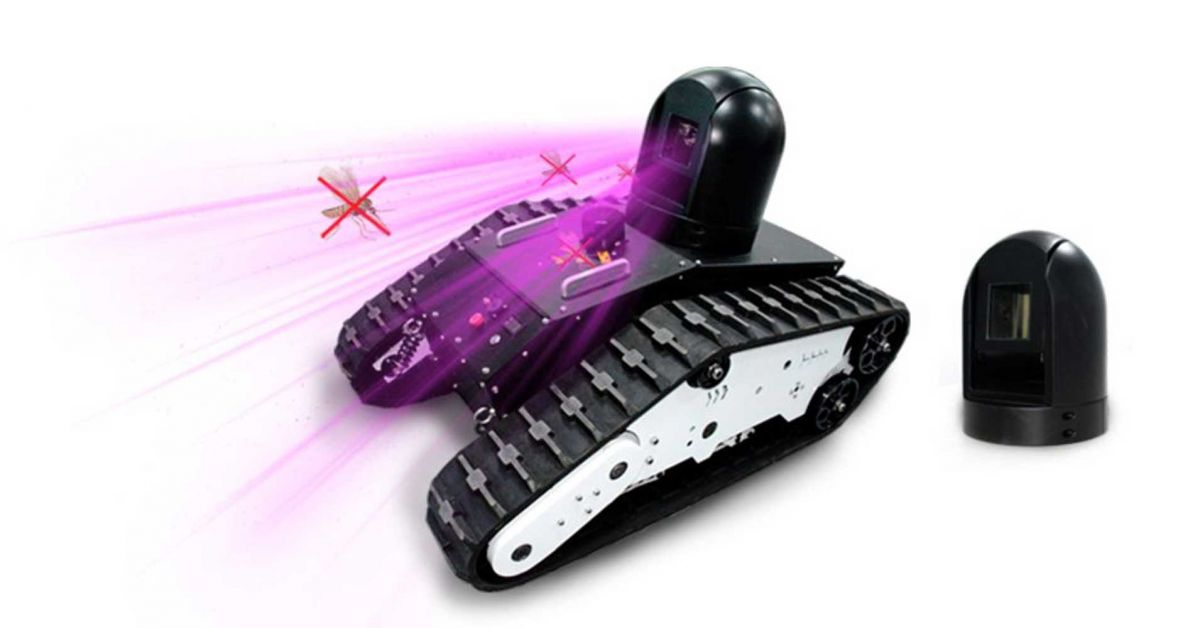
\includegraphics[width=0.8\linewidth]{robot.jpg}
			
		\end{figure}
	\end{center}
	
	This robot has been referred to as a toy-sized autonomous mosquito zapper, designed by a company named LeiShen. Although there is not much information on this whether this robot has actually been deployed or what kind of components it uses, this robot is similar to the project's aim.
	
	
	\subsection{Autonomous Roomba}
	\begin{center}
		
		
		\begin{figure}[H]
			\centering
			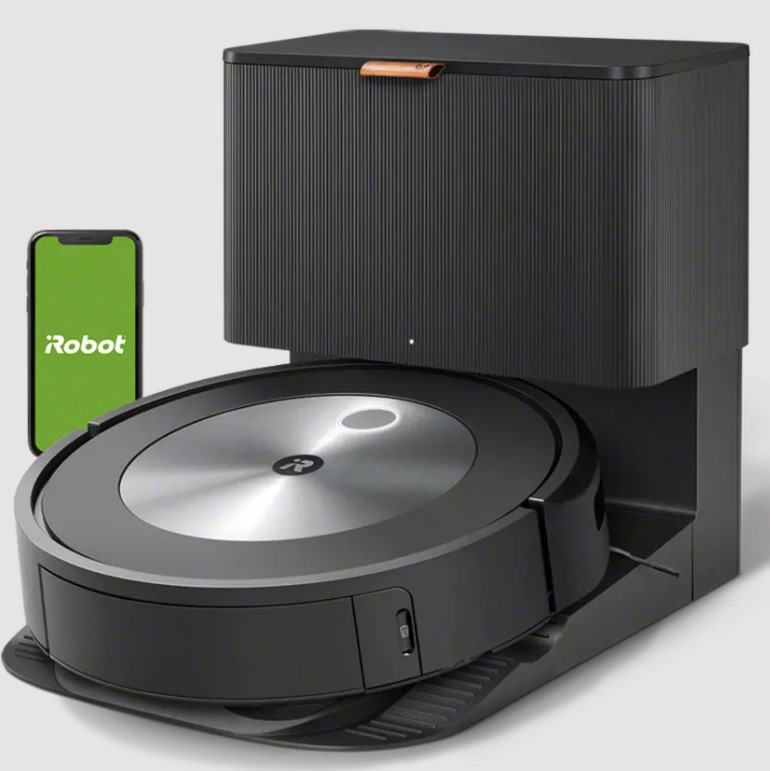
\includegraphics[width=0.46\linewidth]{robot2.jpg}
			
			\label{fig:Robot}
		\end{figure}
	\end{center}
	
	Although a robot vacuum is different from a cockroach annihilator the concept is similar. This cockroach annihilator should be able to roam around room autonomously just like the vacuum and avoid obstacles or have a hard encasing to control damage on the hardware.  
	\section{Challenges}


	
	\subsection{OpenCV}
	
	In one similar experiment, it was found that using OpenCV solely to using a tracker function to track the movement of a mosquito in different methods did not give the greatest results. 
	\begin{center}
		
		
		\begin{figure}[H]
			\centering
			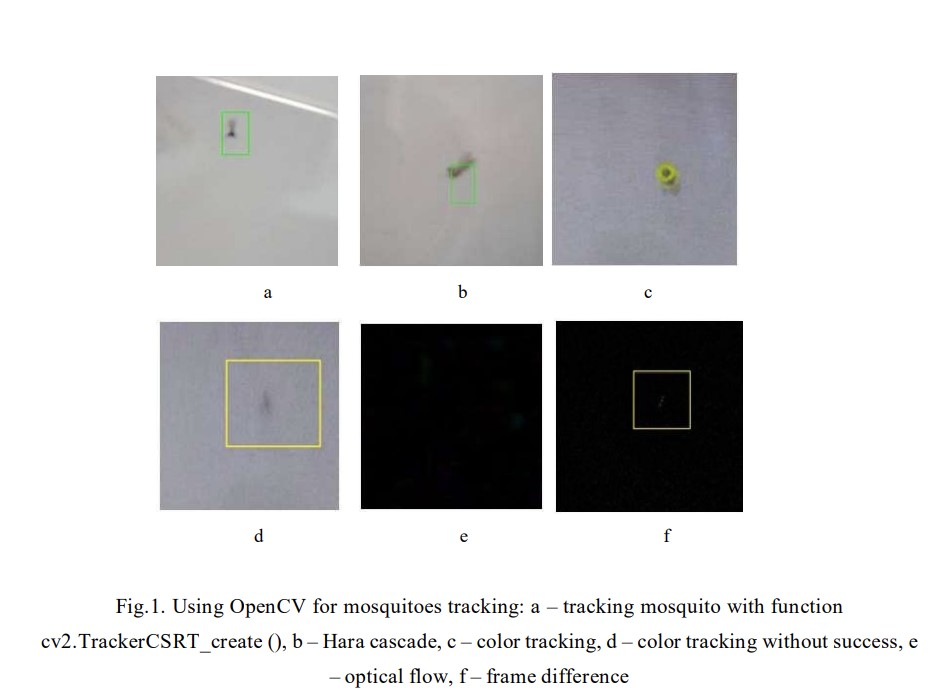
\includegraphics[width=1\linewidth]{opencv.jpg}
			
			\label{fig:opencv}
		\end{figure}
	\end{center}
	As seen in the figure above the mosquito in one of the methods cannot be detected at all, however by using an image processing function called Thresholding ON A 2-4mm sized mosquitoes gave drastically different results:\cite{rakhmatulin_2021_raspberry}
	
	
	\begin{center}
		
		
		\begin{figure}[H]
			\centering
			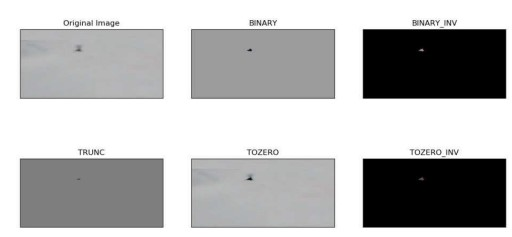
\includegraphics[width=0.8\linewidth]{opencv1.jpg}
			
			
		\end{figure}
	\end{center}
	
	
	
	
		\subsection{Voltage issues}
		When running the code to test the motors it was noted one of the motors failed to work upon further inspection there was immense heat for one of the wires to understand what was happening research indicated there was short circuit using a multimeter we troubleshoot the issue to be wrong wiring.
		
	\subsection{	Angular rotation }



\begin{figure}[H]
	\centerline{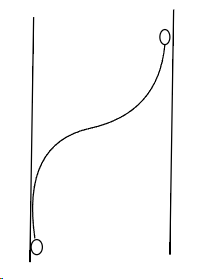
\includegraphics[scale=.8]{angular.png}}
	\caption{Angle bearing example, the curving line represent the smoothness in terms rotation-changing when the robot travels from one circle to the other.}
	\label{stft_figure}
		\end{figure}   
	
	The first concept that was going to be used was angular bearing to rotate the robot in a way that would lead the robot from one point to another in a smooth way. This would be done through the raspberry pi sending the route with the angular motion in between, which is the whole idea behind making this robot move in a smoother manner.
	
	
	However, this was just the first concept, it didn't go as planned due to the robot chassis having an uneven weight distribution. The uneven distribution issue has been further explored and solved in Section \ref{pwm-weight-section}. But to briefly summarise the issue, the uneven weight distribution wasn't the sole problem that was causing this, there were other issues that were also a factor in the execution of implementing bearing angular rotation. Instead, we went with an alternative solution using pulse width modulation which uses time delays in between small motions to have better control from the code


Instead a better alternative for Raspberry pi with a slow processor the robot has been coded to have a higher speed to get up close tot he detected cockroach when the robot is far from cockroach and make micro adjustments in essence smaller bursts of speed when the robot happens to be closer to the cockroach.

There is a disruption in the direction that the robot moves in a higher speed, due to the imbalance in the weight distribution causes a discrepency in speed between the motors. To solve this issue, in the code provided at the end of this report, starting from like 106, the function named "backwards" has been written to amend the discrepency in speed. The discrepency is being eliminated by reducing the speed of one wheel to the point where it matches the speed of the other wheel and make it balanced. A percentage reducer has been implemented in the code which allows the speed of one wheel to be reduced by that percentage, taking into account the constant speed of the other wheel, which prevents the robot from steering into other directions.

The percentage value has been calculated to an approximation using trial and error in the lab. The number that was determined to be the optimal through visual testing was 14.3\%.



	
	\subsection{	Physical Hardware    }
	 Soldering to connect wires is not always a viable option, to solve this extenders were used to, this allowed to connect and disconnect wires that are soldered on the other end without having to shorten the wires. It made this project more time efficient.
	
	Configuring 7 components one  single level robot chassis was not an option especially with the amount of wiring everywhere as time was not at advantage even if a new chassis were to be bought it would be time consuming to strategise component placement to maximise space, so therefore an acrylic board was taken into the workshop, holes were made to align the foundation level. Longer screen and bolts were gifted by the universities workshop which were used to create a space in-between the two levels so that the big batteries could be fitted
	
	
	
	\section{Hardware structure}
	
	
	\begin{center}
		
		
		\begin{figure}[H]
			\centering
			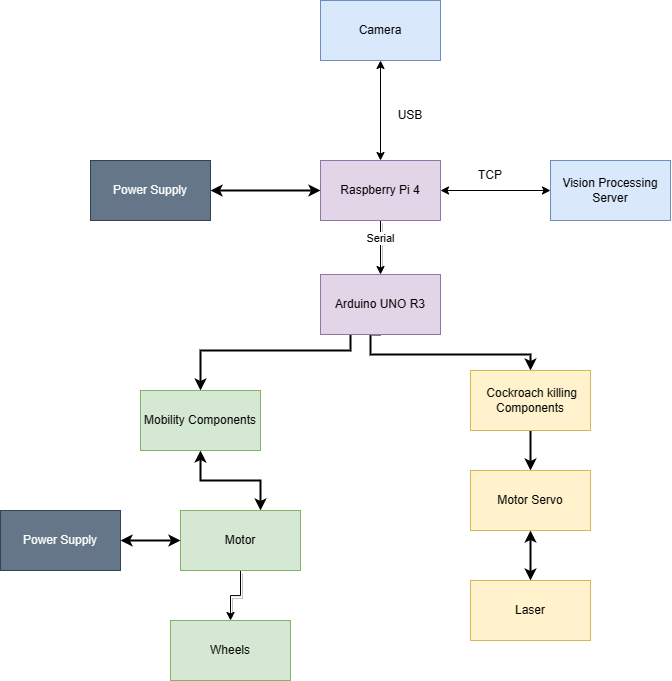
\includegraphics[width=1\linewidth]{high.png}
			\caption{A high level diagram of the robot. }
			\label{fig:robot}
		\end{figure}
	\end{center}



	
	Components requiring to carry out high level task have either User Datagram Protocol (UDP) connection or Gigabit Ethernet, this is to minimise the risk of loosing importance of data due to the speed, if the perception component which is the initialising component  fails to deliver the right data on time it makes the robot ineffective at detecting the cockroach hence unable to annihilating cockroaches, however UDP allows missing packets given this is not a viable option when detection small moving cockraches the better option for the camera is Gigabit Ethernet a USB connection was used instead .Although the Rapberry Pi is connected to the internet so users can visualise what the webcam's field vision is, UDP was not a viable option as it made the data processing unstable on both ends, therefore TCP was used was used. TCP on the other hand is slightly lenient as although it is a slower method of sending data it is guaranteed that the data will be received however this created a backlog of frames due to raspberry pi's slow processing. Serial is the form of connection that has been used towards the lower level tasks such a movement and eliminating cockroach.
	
	
	
	In this project single boards have been used to control components. Rapsberry Pi was used used for the vision component (Webcam), this single board has be chosen as its overall performance is convenient than most other computers due to its availability and its compactness, this is especially important if good resolution and high detection performance is required. The connection between the components was decided based on efficiency and requirement, TCP has been used for two reasons, one of them being less unstable and that the data although slowly guaranteed to be received. In this report the solution to latency in receiving the data is briefly touched on.\ref{Tcp} In the following table a comparison is made between two controllers:

	\begin{center}
		\setlength{\tabcolsep}{10pt} % Default value: 6pt
		\renewcommand{\arraystretch}{1.5} % Default value: 1
		\begin{tabular}{ | m{3cm} |m{3cm} | m{4cm}|  } 
			
			\hline
			& Jetson Nano & Raspberry Pi 3A+   
			\\ 
			
			\hline
			
			GPU & 128-core NVIDIA Maxwell & Broadcom VideoCore IV  \\ 
			
			\hline
			CPU
			& 1.4 GHz 64-bit Quad-Core ARM Cortex-A57 MPCore & 1.4 GHz 64-bit quad-core ARM Cortex-A53
			
			\\ 
			\hline
			
			
			\hline
			RAM
			
			
			& 4GB LPDDR4 &
			512MB LPDDR2 SDRAM
			
			\\ 
			\hline
			
			Video Output: & HDMI, DisplayPort (4K) & HDMI, Display Serial Interface (DSI)
			\\ 
			\hline
			Camera Serial Interface (CSI) & Yes & Yes\\ 
			\hline
			
			
			
			\hline
			Price (CSI) & £154.50 & £54.99\\ 
			\hline
		\end{tabular}
	\end{center}
	
	
	
	For the central computer, Raspberry Pi 4 will be used as an affordable option as although its purpose is to carry out high level planning it does not require to use a lot of resources to carry out tasks.
	
	
	Lastly the microcontroller, Arduno UNO R3, provides a range in terms of needs, it can provide sufficient memory to have good performance in terms of motion control.The microcontrollers provides from 32 Kbytes Flash, 2  Kbytes of SRAM. It's good performance in terms of connectivity, power, efficiency and light-weightlessness is the reason for choosing this microcontroller.
	
	
	
	\subsection{Simultaneous localization and mapping}
	There are three steps in making a model functioning when implementing Simultaneous localization and mapping (SLAM) :
	\begin{itemize}
		\item Perception - To achieve a model of the environment in which the robot will navigate in sensory components such as Lidar can be used, to do detect the mosquito a camera can be used with openCV. Ideally an ultrasonic sensor would be used in the case that the Lidar fails, this type of sensor is deemed useful if the object's vicinity is close.
		\item Planning - consist planning how the autonomous interaction between the computers are going to take place without human interaction, to achieve this a high level central computer is going to be used to do high level planning and receive interfaces from the implementation of perception (Lidar and Camera). 
		\item Action - Low level controllers is going to be used to control the encoders to move around the mapped environment and change the angle as well as direction of the laser.
	\end{itemize}
	\subsection{Key Hardware Components }
	\begin{itemize}
		\item An image processing computer such as raspberry pi was used to visualise and detect the cockroach, an estimated direction up-close to the cockroach will calculated and sent to the Arduino.
		\item The purpose of the Arduino R3 is to get the directions and change motor directions, and receive further calculations to reposition itself until the the lasers beam would fall perfectly on the cockroach when turned on.
		\item 	A high resolution camera is required to detect the size of a cockroach averaging the size of 0.5 to 1 cm, to configure the webcam it was ensured that the view from where the camera is placed is  clear and allows a wide view of the field towards the floor where cockroaches are most likely to be. The preferred frame rate per second should be 30, . Given only one computer is invested to solely receive data from the webcam to process the image, a fast and high quality camera as well as computer  such as the Jetson Nano Computer would have been more ideal to process the frames as challenges faced using raspberry pi will be explored throughout the report.
		
		\item A laser strong enough to neutralise a mosquito however weak enough to not harm the human eye would be ideal to  make this robot safer, to configure the laser according the camera's coordinates of the laser has been attached to a Servo motor before it is fixed on the robot.
	
		
		
	\end{itemize}
	
	\subsection{Steps in Connecting the Hardware}
	
	
		\begin{center}
		
		
		\begin{figure}[H]
			\centering
			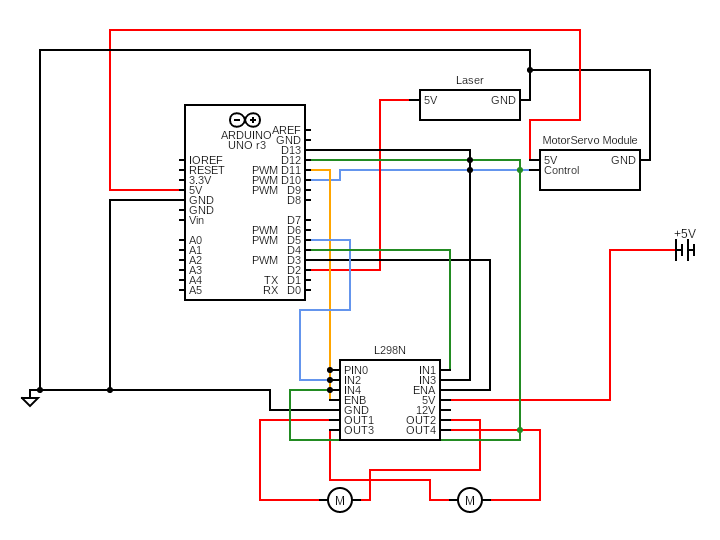
\includegraphics[width=1\linewidth]{circuit.png}
			\caption{A circuit diagram of the robot.  }
			\label{fig:Flowchart}
		\end{figure}
	\end{center}
	
	
	The camera will raspberry, upon receiving a location and movement information input the Arduino can use the data to adjust the robots motor and as for the laser is attached to the motor servo and that is fixed when the robot is switched on.
	

	
	
	The laser connected to the servo motor or robotic arm should then be connected to the control system with the right cables, the purpose of the laser is aim and eliminate cockroach detected from a calculated direction from the coordinates received from the camera.
	
	To ensure the system is working the circuit should be tested at this point and make further adjustments.
	One adjustment required will be the calculation of the laser's's aim when pointing at the cockroach, this is going to be dependant on the robot's design in terms of size and distance from the camera. To detect cockroaches the webcam is going to use image processing function, given the placement of the laser and the webcam  on the chassis is going to be different from each other, the camera's coordinates on the detected cockroaches is not going to allow the laser to aim correctly, therefore an angle direction will be need to be adjusted in the servo motor to point the laser correctly.
	
	
	To calculate this, the angle at which the servo motor needs to move the laser is required. This can be done using basic trigonometry, by calculating the angles formed by the lines connecting the center of the camera's field of view, the location of the detected mosquito, and the servo motor axis.
	

		\section{Pulse Width Modulation} \label{Tcp}
		
		\label{pwm-weight-section}
	
	In this section the method used to detect and control speed using PWM will be discussed, the purpose of controlling speed is being able to stop or slow down to accommodate parking up-close to the cockroach so that the laser-beam sits directly on top of the detected cockroach. The power supply would pulse the motors  High or Low in other terms on and off at a certain frequency at a specific pulse width to control the speed of the motors.
	
	The initial idea behind using the PWM method was to control speed and slow one of the motors off to turn left or right, the voltage is directly in proportion to the width of the pulse, the term for this is called duty cycle. The general understanding is that the if the higher the duty cycle meaning the more there is pulse width the more increased the speed will be. There has been a  slight changes to the initial idea as we progress into the execution of this robot due to the uneven distribution which is later fixed and explained under the section challenges in this report.
	
		\begin{center}
		\begin{figure}[H]
			\centering
			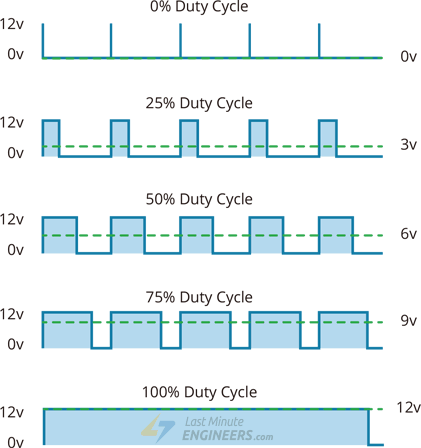
\includegraphics[width=0.42\linewidth]{pwm.png}
			\caption{PWM duty cycle- the higher the duty cycle the more increased the duty cycle will be.  }
			\label{fig:Flowchart}
		\end{figure}
	\end{center}

	Initially to control speed an l293D motor driver chip was used to control the speed, once set up it was noted that this type of single chip without a module would require too many wires.
	
\begin{center}
	\begin{figure}[H]
		\centering
		\subfloat[\centering The L293D module at hand ]{{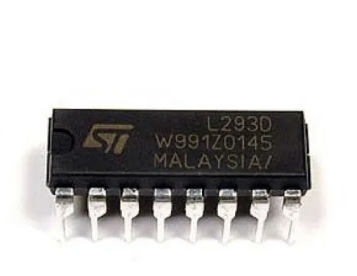
\includegraphics[width=0.45
				\linewidth]{L293D.PNG} }}%
		\qquad
		\subfloat[\centering The wiring management required to using the component]{{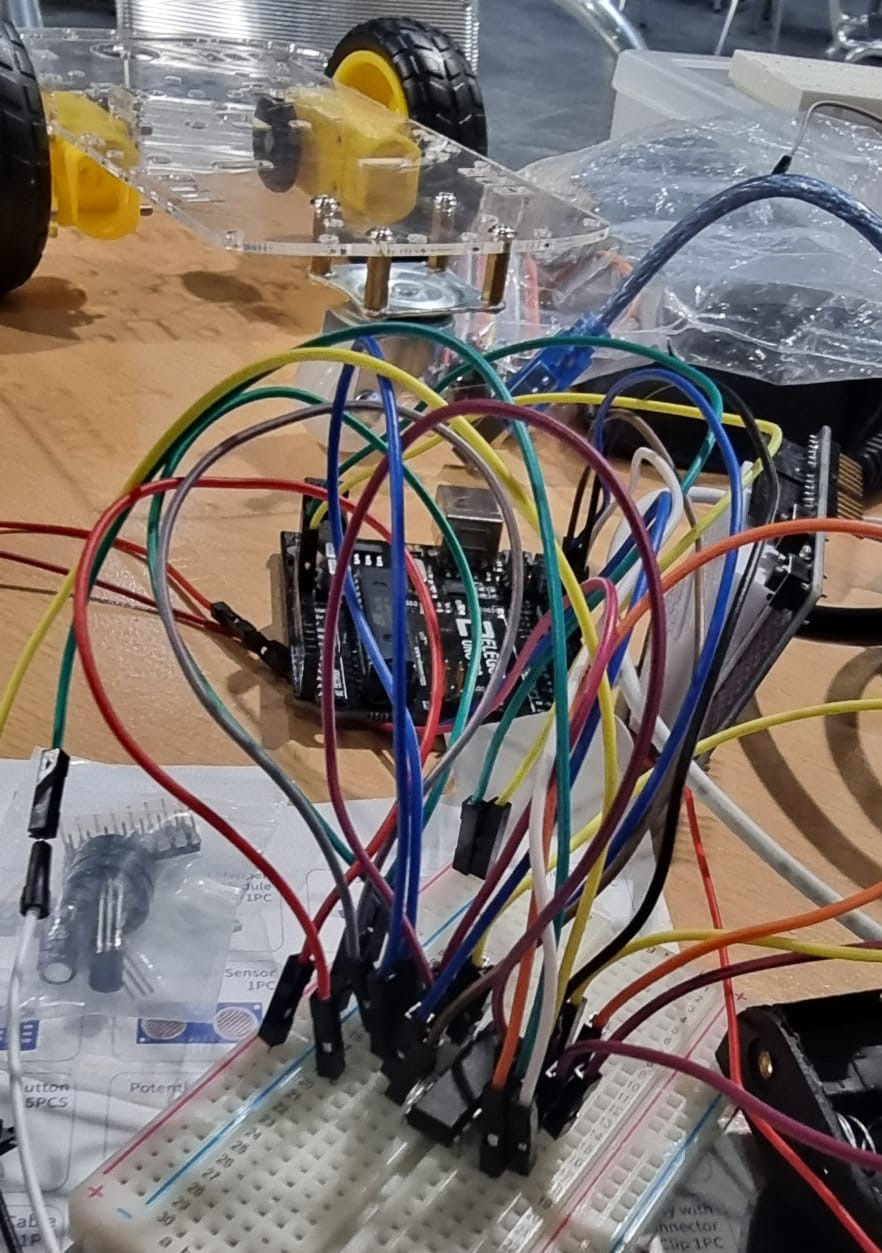
\includegraphics[width=0.40\linewidth]{l293d.jpg} }}%
		\caption{Using L293D module to control the motor driver.}
		\label{fig:Starting}
	\end{figure}
	
\end{center}



This was inefficient as valuable space would be compromised if a breadboard is included on the chassis. Upon further research another module called L293N was found under whose specification allowed us to use PWM.

\begin{center}
	\begin{figure}[H]
		\centering
		\subfloat[\centering The motor driver installed in the robot]{{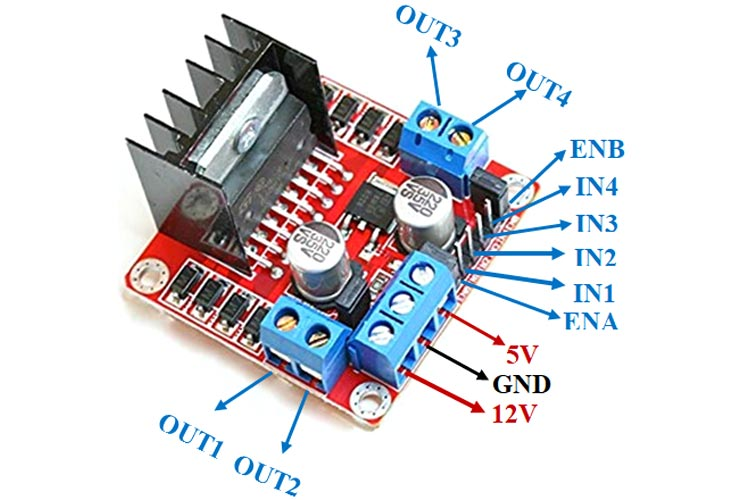
\includegraphics[width=0.50
				\linewidth]{l293n.jpg} }}%
		\qquad
		\subfloat[\centering The wirings have been braided to shorten their length and to have a neater and dcipherable appearance]{{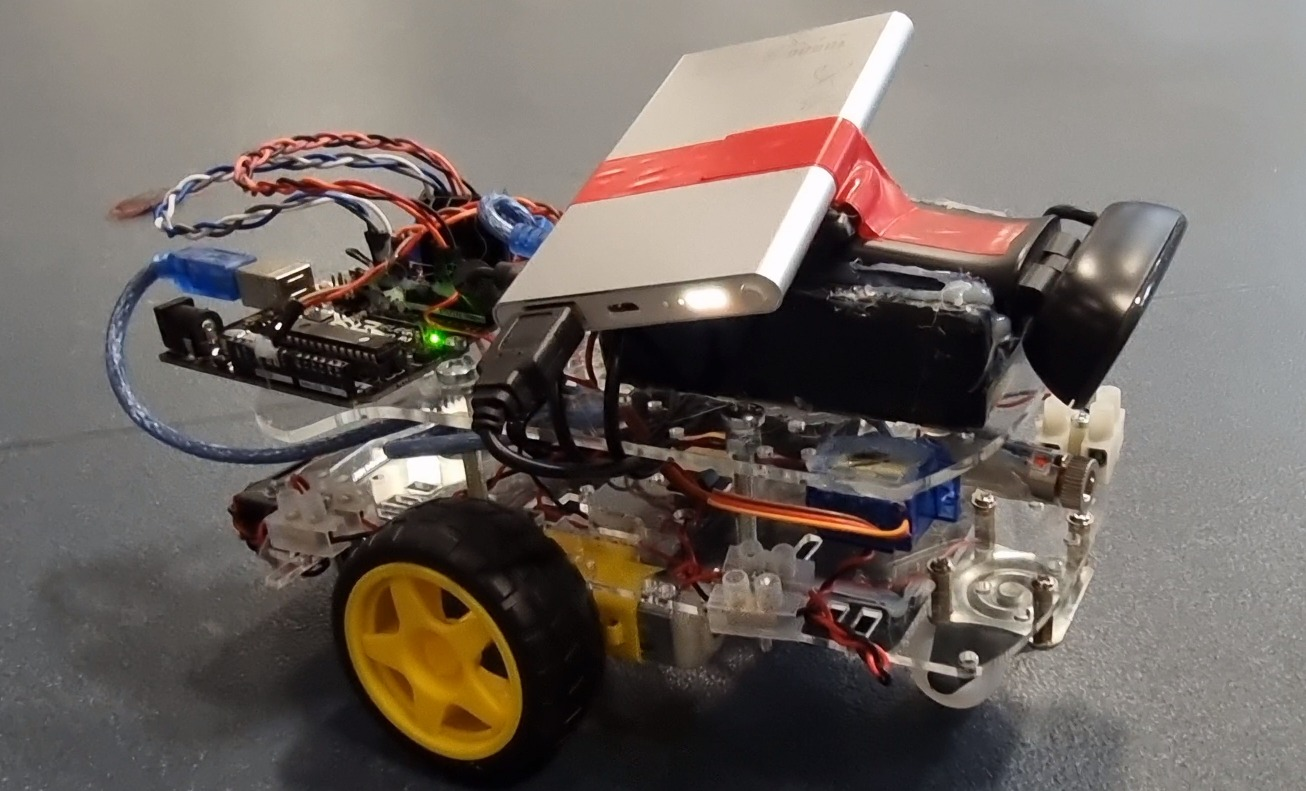
\includegraphics[width=0.40\linewidth]{wiring.jpg} }}%
		\caption{The wiring after including a motor driver }
		\label{fig:Starting}
	\end{figure}
	
\end{center}
The table below has been designed to understand what the purpose of each pin is 
	\begin{center}
	\setlength{\tabcolsep}{10pt} % Default value: 6pt
	\renewcommand{\arraystretch}{1.5} % Default value: 1
	\begin{tabular}{ | m{3cm} |m{11cm} |  } 
		
		\hline
		Pins & Purpose   
		\\ 
		
		\hline
		
		OUT1, OUT2 \& OUT3 OUT4 & Each side will control the amount of  power supplied on each side; Motor A and motor B.  \\ 
		
		\hline
		5V \& GND \& 12V 
		& are required to power the motor 
		\\ 
		\hline
		
		
		IN1, IN2 \& IN3, IN4 
		
		& The purpose of these four pins is to control direction where in1 and in2 would be responsible for motor A, In3 and in4 would control the spinning direction of motor B. The code for for each direction are provided in the appendices starting form line 133-206 \ref{code}
		
		\\ 
		\hline
		
	
		
	\end{tabular}
\end{center}



	
The initial idea entailed stopping or slowing one motor in order to turn into a clock-wise right direction and vice versa when turning left. 


However this idea was put onto halt after realising that direction of would slight change when going slightly to the left or right which would lead the cockroach to be out of the frame. An important note to be made is that, even when moving forward the robot was unable to keep straight and rather fo into an angle. To troubleshoot this several assumptions were made:
\begin{itemize}
	\item The front wheel is not spherical therefore  when stopping quickly due to the force the front wheel would steer in another direction, changing the wheel was taken out of the equation as there time and financial restraints. This assumption is unlikely unless it involves turning left or right. 
	\item There is uneven weight distribution. Adding the 4 heavy 18650 Lithium batteries at the rear end of the robot caused the weight to be more in comparison to the front, this lead the robot to tilt backward when going at a higher speed changing the direction of the front wheel, to fix this weight have been added at the front by using a battery holder of four AA batteries, but this was not a perfect a solution it was decided that there would be a reduction in speed in one of the motors of around 14.3 percent.
	\item	There is an OpenCV issue of  backlog of frames due to raspberry pi being not fast enough to process them therefore giving direction even though cockroach is no longer in the frame. To amend this a few frames are deleted to have a updated queue of frames.
\end{itemize}


Generally speaking, this could have been solved in a more efficient manner had there been more time and the finance to fund for better resources.


	
	\section{Software}
	
	
	\begin{center}
		
		
		\begin{figure}[H]
			\centering
			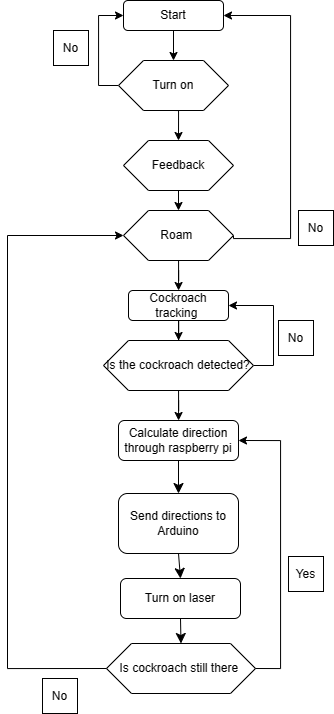
\includegraphics[width=0.5\linewidth]{flaw.drawio1.png}
			\caption{A flowchart of the steps involved in the robot. }
			\label{fig:Flowchart}
		\end{figure}
	\end{center}
	
	
	Image processing algorithms  was used to automatically detect and track cock in the camera's field of view. This can be done using techniques such as threshold, edge detection, and object recognition algorithms.
	
	The detected cockroach would then be identified using  their location and movement direction, and use this information to control the robot's movements and aim the laser when robot is close to the cockroach.
	
	Lastly the laser would be fired at the detected cockroach, using the robot's aiming mechanism, to kill them on contact.
	
	
	To make the laser move according to the camera, a servo has been used or in a much more scaled up project robotic arm to aim the laser. In this case the servo motor can be controlled by the robot's control system, using the location and movement information of the detected cockroach provided by the camera and image processing algorithms.
	
	The control system would use the location of the detected cockroach to calculate the necessary angle and direction for the servo motor or robotic arm to move the laser. This information was then be sent to the servo motor, which would move the laser to the desired position however this was to complicated to carry due to the uneven weight distribution steering the wheel away.
	
	Therefore fixing laser and positioning the webcam along with servo motor that is holding the laser in such a way that the laser is always aimed at the centre of the camera's field of view. In this way the Raspberry Pi can adjust the robot to keep the laser pointed at the cockroach even if the cockroaches were to move.
	


\subsection{ Establishing communication}




\begin{lstlisting}[style=myArduino]
	void parseCommand() {
		if (command[0] == '1') {
			String timesToRunString = command.substring(1, 4);
			int timesToRun = timesToRunString.toInt();
			forward(timesToRun);
		} else if (command[0] == '2') {
			String timesToRunString = command.substring(1, 4);
			int timesToRun = timesToRunString.toInt();
			backward(timesToRun);
		} else if (command[0] == '3') {
			String timesToRunString = command.substring(1, 4);
			int timesToRun = timesToRunString.toInt();
			right(timesToRun);
		} else if (command[0] == '4') {
			String timesToRunString = command.substring(1, 4);
			int timesToRun = timesToRunString.toInt();
			left(timesToRun);
		} else if (command == "5") {
			startLaser();
		} else if (command == "6") {
			stopLaser();
		} else if (command[0] == '7') {
			String angle = command.substring(1, 4);
			int angleInt = angle.toInt();
			changeLaserAngle(angleInt);
		}
	}
\end{lstlisting}


Given to establish communication the commands were parsed from Raspberry Pi to Arduino, to make processing more efficient due to the Pi's slow processing nature instead of putting string commands into an array of characters and processing it the first digit of the four numbers have been used to indicate the direction the robot should turn. Therefore if the number is one  then the robot should be running the forward function.

After doing so the next set of three digits would need to be processed. The table below displays how Raspberry Pi establishes and sends commands to the Arduino.

	\begin{center}
	\setlength{\tabcolsep}{10pt} % Default value: 6pt
	\renewcommand{\arraystretch}{1.5} % Default value: 1
	\begin{tabular}{ | m{3cm} |m{11cm} |  } 
		
		\hline
		 Command & Function   
		\\ 
		
		\hline
		
		1xxx & Run the motors forward with the speed of 
		“xxx”. Therefore, a command of “1010” will 
		send forward with a speed of 10. The same 
		format is being used for all movement 
		commands   \\ 
		
		\hline
		2xxx
		& Run the motors backwards.
		
		\\ 
		\hline
		
		
	
		3xxx
		
		
		&Right – Run the right wheel motor forward and 
		keep the left one still.
		
		\\ 
		\hline
		
	4xxx & Left – Run the left when motor forward and 
	keep the right one still.
		\\ 
		\hline
		5 & Turn on the laser 
		\\ 
		\hline
		
		
		

		6  & Turns off the laser\\ 
		\hline
		7xxx & Sets the angle of the laser. The xxx can be 
		replaced with the integer for the angle with 
		padded 0s before it such as “7090” will result in 
		a 90-degree angle, or “7180” will result in a 
		180degree angle being set and “7000” will 
		result in 0-degree angle being set
		\\
		\hline
		
	\end{tabular}
\end{center}




What might be notices in the code is that there are two sets forward functions.  

The runMotorForward set the pins to travel the direction ad for the forwards defines how many burst of of high low should the robot carry out while maintaining the same speed the Raspberry pi sent in the he command.

	\section{Component List}
	
	
	
	\textbf{High-resolution cameras} a webcam Logitech C270 HD Webcam was used, its frame rate and good resolution was used be used to capture images of cockroaches and identify them based on their shape and size. To identify cockroaches machine learning has been used to train cockroach detection this would then be used to automatically detect and track cockroaches in real-time.
	
	
	
	\begin{center}
		
		
		\begin{figure}[H]
			\centering
			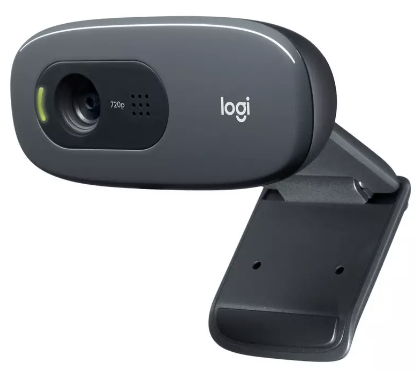
\includegraphics[width=0.5\linewidth]{webcam.png}
			\caption{Webcam:  Logitech C270 HD Webcam used to detect and track cockroaches in the robot's field of view.}  
			\label{fig:Flowchart}
		\end{figure}
	\end{center}
	
	
	
	
	\textbf{Servo motor }: A servo motor, such as the Tower Pro SG90 or the DYNAMIXEL AX-12A was  used to have a fixed aim the laser at the detected cockroach the angle of rotation is fixed upon starting each time if changed.
	\begin{center}
		
		
		\begin{figure}[H]
			\centering
			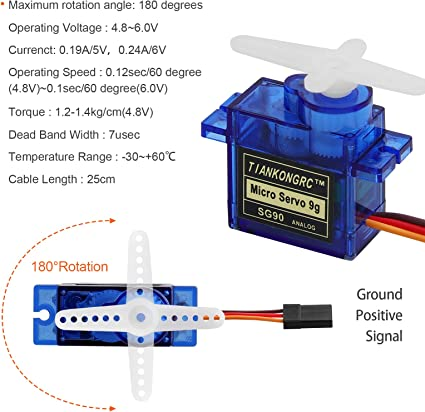
\includegraphics[width=0.5\linewidth]{motor.jpg}
			\caption{SG90 9g Micro Servos for RC Robot used to control the laser's pointing angle.}  
			\label{fig:Flowchart}
		\end{figure}
	\end{center}
	
	
	
	\textbf{Laser}: A laser, WayinTop 650 nm Focusable Focus Adjustable Lens Laser Red Line Diode Module 3-5V Driver was used be used to point at the  the detected cockroach. A laser, or other high-intensity light source such as the 445nm Blue Laser Module or the 532nm Green Laser Module, that is capable of killing cockroaches on contact would be more suitable for this project but due to financial restraints the laser below was used.
	
	\begin{center}
		
		
		\begin{figure}[H]
			\centering
			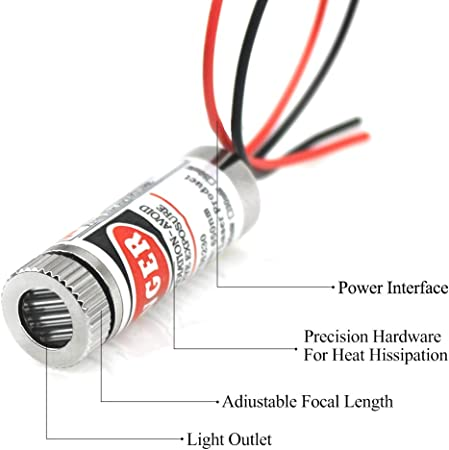
\includegraphics[width=0.5\linewidth]{laser1.jpg}
			\caption{High Power 445nm Focusing Blue Laser Module Laser Engraving}  
			\label{fig:Flowchart}
		\end{figure}
	\end{center}
	
	\textbf{Control system}: A control system, Raspberry Pi 4,  was used to process the input from the camera, the purpose is to process the input from the cockroach detection system and send this to information on direction to Arduino.
	
	\begin{center}
		
		
		\begin{figure}[H]
			\centering
			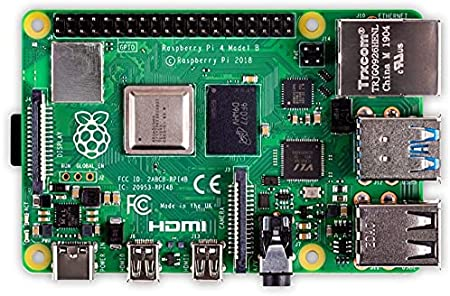
\includegraphics[width=0.5\linewidth]{ard.jpg}
			\caption{ Raspberry Pi 4 Model B 8GB }
			\label{fig:Flowchart}
		\end{figure}
	\end{center}
	
	The decision of using following computers have been explained in the hardware section.
	\begin{center}
		
		
		
		
		\begin{figure}[H]
			\centering
			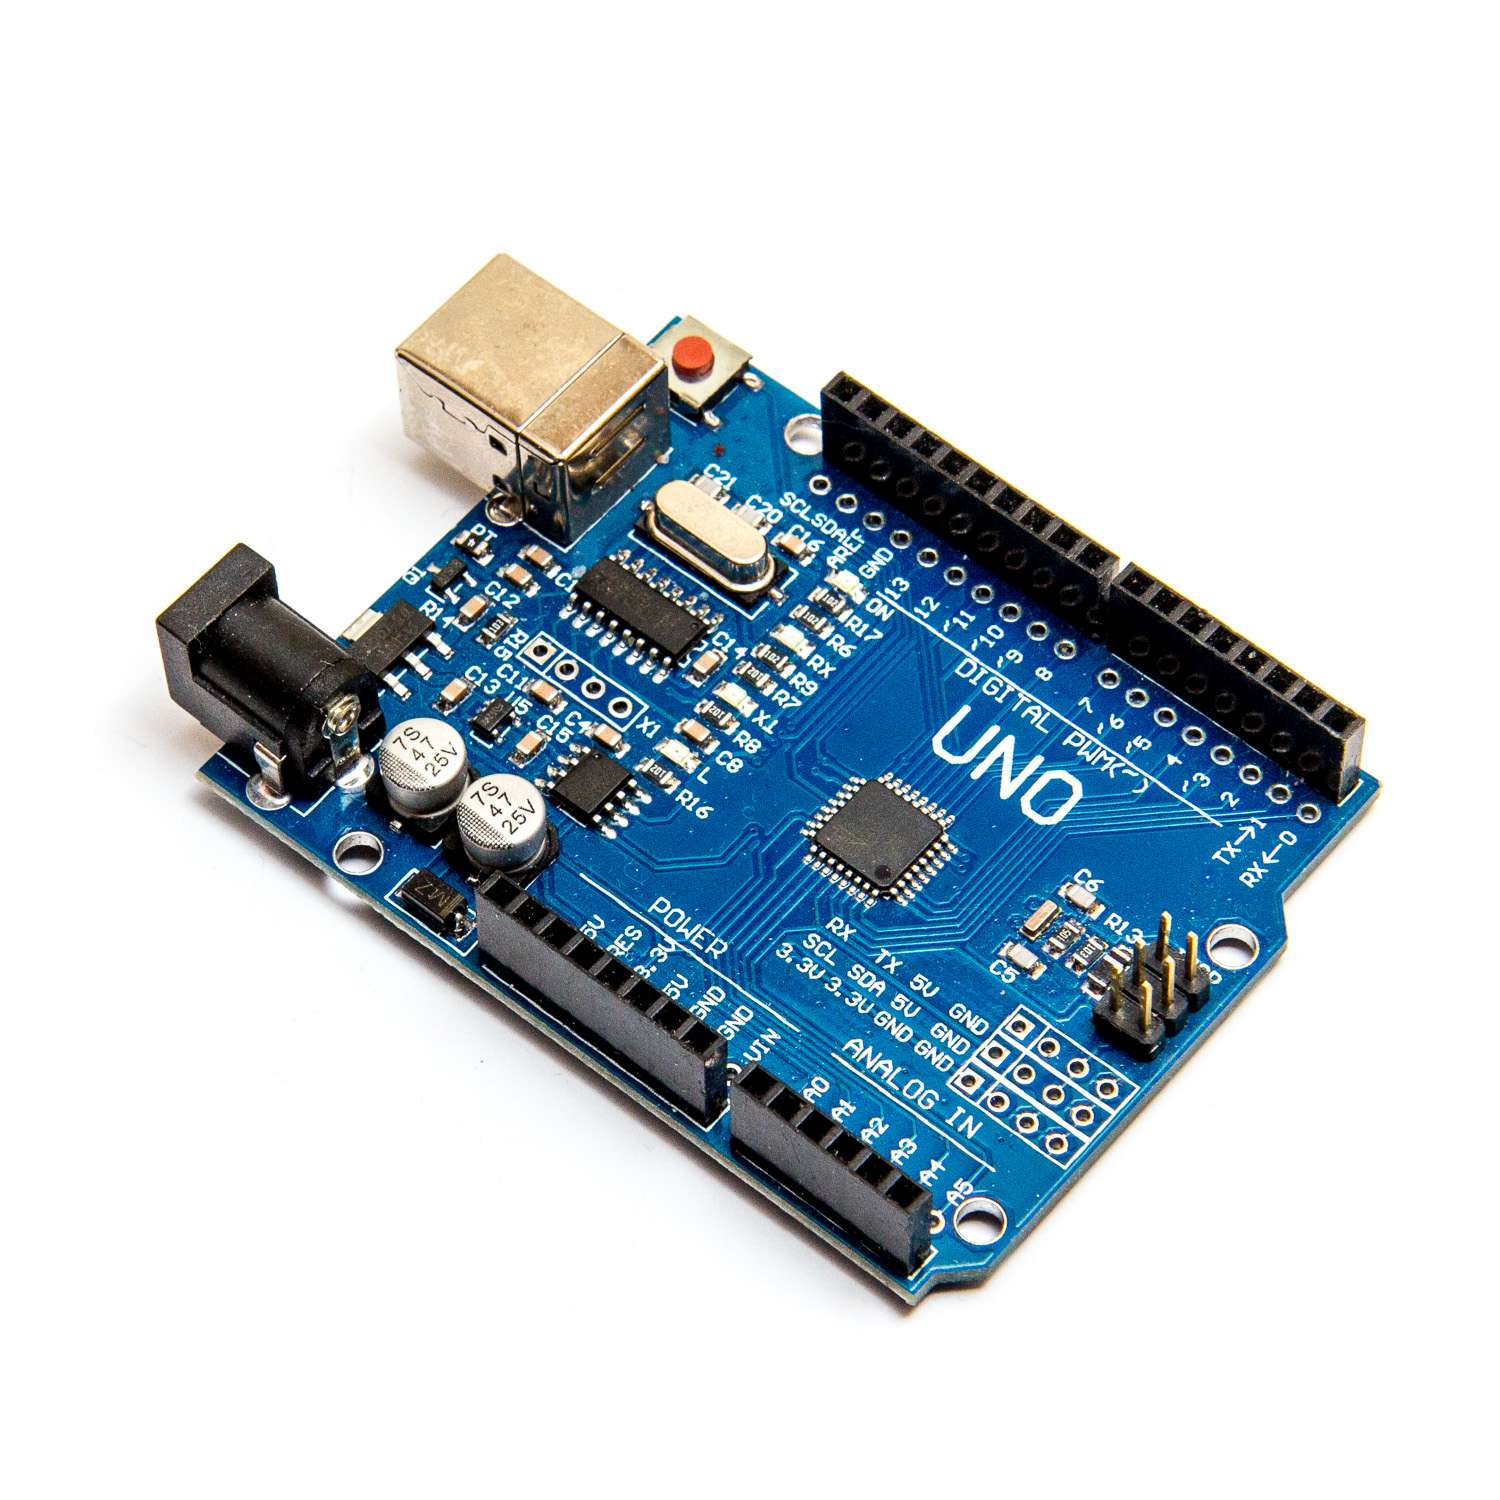
\includegraphics[width=0.5\linewidth]{arduino.jpg}
			\caption{ Arduino UNO R3 }
			\label{fig:Flowchart}
		\end{figure}
	\end{center}

		
		
		
			\textbf{Microcontroller}:An Arduino UNO R3 was used receive commands from the Raspberry Pi to control the motors direction and fire the laser. The motor servo's angle is configure upon starting the robot.
			\begin{center}
			
			
			\begin{figure}[H]
				\centering
				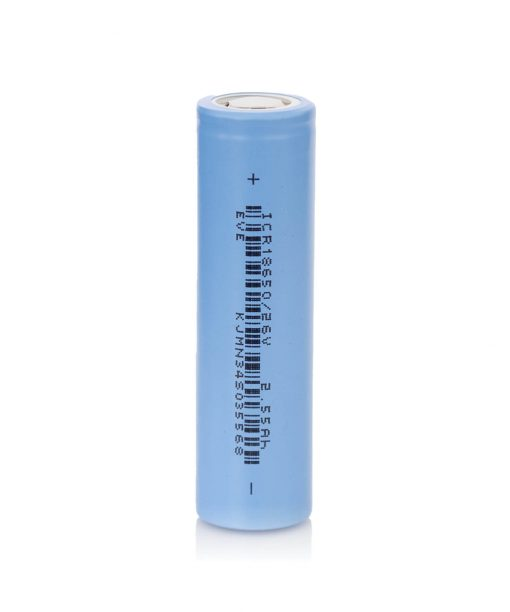
\includegraphics[width=0.4\linewidth]{batteries.jpg}
				\caption{  18650 EVE Lithium Ion LI-ION Rechargeable 3.7V 2600mAh Battery }
				\label{fig:Flowchart}
			\end{figure}
		\end{center}
	
	
	\textbf{Power supply}: A power supply, 18650 EVE Lithium Ion LI-ION Rechargeable 3.7V 2600mAh Battery was used as 4 of them gave enough voltage to run the motor driver and the two motors and advantage of using these batteries is that they are rechargeable, a power bank was used to power Raspberry Pi. These can then be used to provide the necessary electrical energy for the circuit.
				\begin{center}
	
		\begin{figure}[H]
		\centering
		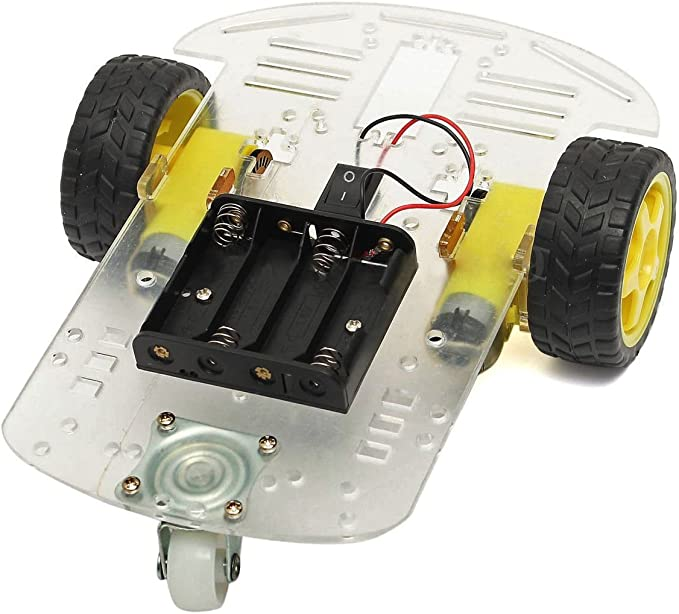
\includegraphics[width=0.4\linewidth]{chassis.jpg}
		\caption{ A three wheeled robot chassis.   }
		\label{fig:Flowchart}
	\end{figure}
\end{center}
	\textbf{	A housing or chassis} to hold and protect the other components, and provide a way for the robot to move around and access areas where cockroach may be present.
	
	In addition to these core components, additional hardware such as soldering machine, Jumper cables, Extenders, an acrylic board to create a second level were required to complete this project.
	
	\section{Safety Protocol}
	
	To make sure that cockroach annihilating robot is safe to operate, the following steps can be taken as precaution:
	\begin{itemize}
		\item 	Using appropriate wiring and connectors should ensure that the connection is strong and can be used with the appropriate voltage, there are few ways to notice faults which include if the wire is heating up there maybe a shortage one can check the readings on a multimeter and the components specification to get a better understanding, in another instance one motor maybe failing to work due to not enough volts, this can be checked using tools that allows checking how much voltage is enough to run both motors.
		\item 
		Although fuses have not been used in this project in a real scenario where this robot would be used as a household item, fuses or circuit breakers may be required to prevent potential hazardous malfunctions such as excessive current or a short circuit.
		\item To ensure the right voltage is being used in the circuit using appropriate power sup-plies and voltage regulators should be used to prevent hazardous situations, this can prevent potential damage within the components and ensure the robot is operating at its optimal.
		\item Using heat sinks and other cooling techniques should be able to prevent components from overheating, this can help components getting rid of excessive heat and operate components under safe temperature.
		\item And lastly the circuit must always be tested before operating to make sure the robot would function properly and safely.There's a variety of equipment available to test this including but not limited to multimeters.
		
		
		
	\end{itemize}


	
	
	Following the steps above can ensure the cockroach annihilating robot's circuit is safe to operate.
	
	
	
	
	\section{Further Development}
	
	After the robot one issue remained with connecting the raspberry pi to the internet and reconfiguring the ip address, to fix this programming the the raspberry pi to automatically connect would make the setting up process a much faster.
	
	
	More than one sensor can be used to detect cockroaches more accurately, this can include:
	
Developing and using a more complex algorithms to detect cockroaches, and track their movement, as the current robot does not track moving cockroaches. Implementing a cockroach tracking robot that can detect cockroaches in different kinds of environment  would make the robot more efficient and improve its detection accuracy.

Implementing obstacle avoidance by using LIDAR/SLAM or ultrasonic sensors may help the robot navigate without damaging itself would be make it suitable to operate in real environments where the are object and people. 

To further develop this robot, efficiency in terms of power usage can be looked at starting from adding solar panels to reserve energy in public settings, to developing a house the robot can go back when battery is low in a home setting. Adding such power management strategies would greatly enable for the robot to operate longer before having a human checking on its battery health.

Implementing other functions in this robot such as having a insecticide spray attached can help evolve further.

The following part of this section will look more into sensors that this robot can have:
\begin{itemize}
	\item Acoustic Sensors: cockroaches make make certain sounds that may require further research, if detetected by a microphone or an acoustic sensor, such a sensor can be used to detect the exact location of the sensor,if not, it can help verify its presence.

	\item Chemical sensors: Looking into the types of chemicals cockroaches are attracted can be studied. A gas chromatograph which is a chemical sensor can be used to detect these certain chemical and infer the possibility of the presence of cockroaches.
	\item Advancement sensors: Can be used to prevent the robot from crashing into humans and prevent its externals from being damaged.
	
\end{itemize}

	
	\section{Conclusion}

	To conclude, it can be said this with confidence this project has been completed successfully, the each point in the behavioural concept has been met. Overall this group project has been a good practical hands-on experience, from putting ideas into paper to putting a physical hardware have been two very different experiences. This was a steep learning curve, from buying modules to implementing another level on a chassis to allow more spaces. A lot of challenges were faced from calculating the  uneven weight distribution to making the processing of information faster. But in brief this project compared to the proposal which is a similar concept required a lot more planning and a lot of amendments was required. This robot can be considered as a prototype for something very scalable and something that is applicable to real life settings in hopes to the near future.Nonetheless, the concept of automating technology that deals with pests is more than necessary than ever before. 
	
	\begin{center}
	
	
	\begin{figure}[H]
		\centering
		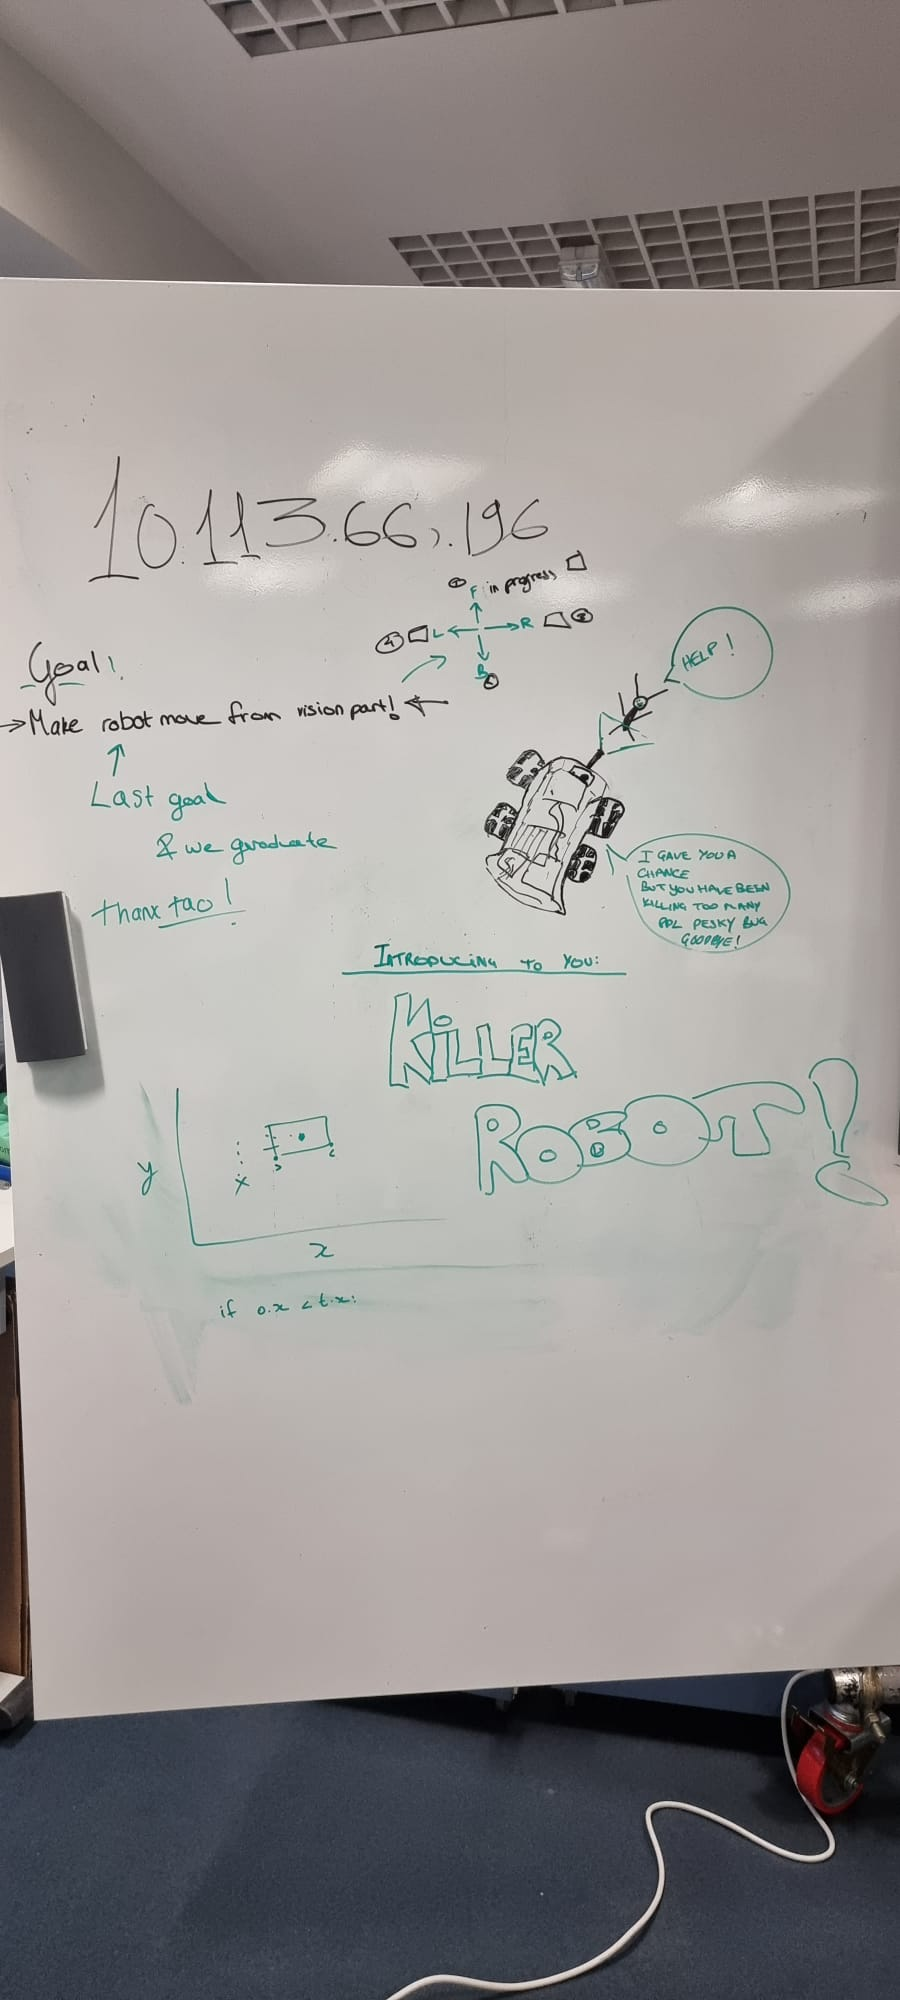
\includegraphics[width=1 \linewidth]{final.jpg}
		\caption{One final message left on the board after getting the robot working  }  
		\label{fig:Flowchart}
	\end{figure}
\end{center}
	
		\section{Code} \label{code}
\begin{lstlisting}[style=myArduino]
#include <Servo.h>


// Motor A connections
int enA = 3; // White
int in1 = 4; // Orange
int in2 = 5; // Purple
// Motor B connections
int enB = 11; // White
int in3 = 13; // Blue
int in4 = 12; // Grey
int servo_pin = 10;
int laserPin = 2; // Red
double rightWheelCurrentSpeed = 0;
double leftWheelCurrentSpeed = 0;


Servo laserServo;
int angle = 40;
int motorServoPin = 4;
int constantSpeed = 75;

String command = "";


void pinSetup(){
	
	pinMode(enA, OUTPUT);
	pinMode(enB, OUTPUT);
	pinMode(in1, OUTPUT);
	pinMode(in2, OUTPUT);
	pinMode(in3, OUTPUT);
	pinMode(in4, OUTPUT);
	pinMode(laserPin, OUTPUT);
	pinMode(motorServoPin, OUTPUT);
	
	// Turn off motors - Initial state
	digitalWrite(in1, LOW);
	digitalWrite(in2, LOW);
	digitalWrite(in3, LOW);
	digitalWrite(in4, LOW); 
	digitalWrite(motorServoPin, HIGH);
	
	laserServo.attach(servo_pin);
}

void setup() {
	pinSetup();
	laserServo.write(angle);
	Serial.begin(9600);
}

// Commands
// 1 - Forward
// 2 - Backwards
// 3 - Right
// 4 - Left
// 5 - Laser on
// 6 - Laser off
// 7 - Laser Angle: usage: 7009 (9 degree)
void loop() {
	if (Serial.available()) {
		delay(10);
		while (Serial.available() > 0) {
			char character = Serial.read();
			command += character;
		}
		parseCommand();
		command = "";
		Serial.flush();
	}
}

void parseCommand() {
	if (command[0] == '1') {
		String timesToRunString = command.substring(1, 4);
		int timesToRun = timesToRunString.toInt();
		forward(timesToRun);
	} else if (command[0] == '2') {
		String timesToRunString = command.substring(1, 4);
		int timesToRun = timesToRunString.toInt();
		backward(timesToRun);
	} else if (command[0] == '3') {
		String timesToRunString = command.substring(1, 4);
		int timesToRun = timesToRunString.toInt();
		right(timesToRun);
	} else if (command[0] == '4') {
		String timesToRunString = command.substring(1, 4);
		int timesToRun = timesToRunString.toInt();
		left(timesToRun);
	} else if (command == "5") {
		startLaser();
	} else if (command == "6") {
		stopLaser();
	} else if (command[0] == '7') {
		String angle = command.substring(1, 4);
		int angleInt = angle.toInt();
		changeLaserAngle(angleInt);
	}
}

void backward(int timesToRun) {
	int backwardSpeed = 85;
	double percentageReduction = 14.3;
	double percentageReduced = (percentageReduction * backwardSpeed) / 100;
	double leftWheelSpeed = backwardSpeed - percentageReduction;
	double rightWheelSpeed = backwardSpeed;
	for (int i = 0; i < timesToRun; i++) {
		runMotorBackward(leftWheelSpeed, rightWheelSpeed);
		delay(25);
		stop2();
		delay(15);
	}    
}

void forward(int timesToRun) {
	double percentageReduction = 2;
	double percentageReduced = (percentageReduction * constantSpeed) / 100;
	double leftWheelSpeed = constantSpeed;
	double rightWheelSpeed = constantSpeed - percentageReduced;
	for (int i = 0; i < timesToRun; i++) {
		runMotorForward(leftWheelSpeed, rightWheelSpeed);
		delay(25);
		stop2();
		delay(10);
	}    
}

void spinIdleRight() {
	analogWrite(enA, 80);  
	analogWrite(enB, 80);
	int timesToRun = 7;
	for (int i = 0; i < timesToRun; i++) {
		digitalWrite(in1, LOW);
		digitalWrite(in2, HIGH);
		digitalWrite(in3, LOW);
		digitalWrite(in4, LOW);
		delay(25);
		stop2();
		delay(25);
	}  
}

void runMotorForward(double leftSpeed, double rightSpeed) {
	rightWheelCurrentSpeed = rightSpeed;
	leftWheelCurrentSpeed = leftSpeed;
	analogWrite(enA, leftSpeed);  
	analogWrite(enB, rightSpeed); 
	digitalWrite(in1, LOW);
	digitalWrite(in2, HIGH);
	digitalWrite(in3, HIGH);
	digitalWrite(in4, LOW);
}

void runMotorBackward(double leftSpeed, double rightSpeed) {
	rightWheelCurrentSpeed = rightSpeed;
	leftWheelCurrentSpeed = leftSpeed;
	analogWrite(enA, leftSpeed);  
	analogWrite(enB, rightSpeed); 
	digitalWrite(in1, HIGH);
	digitalWrite(in2, LOW);
	digitalWrite(in3, LOW);
	digitalWrite(in4, HIGH);
}

void stop2() {
	digitalWrite(in1, LOW);
	digitalWrite(in2, LOW);
	digitalWrite(in3, LOW);
	digitalWrite(in4, LOW);
}

void left(int timesToRun) {
	analogWrite(enA, 80);  
	analogWrite(enB, 80); 
	int timeStarted = millis();
	for (int i = 0; i < timesToRun; i++) {
		digitalWrite(in1, LOW);
		digitalWrite(in2, LOW);
		digitalWrite(in3, HIGH);
		digitalWrite(in4, LOW);
		delay(25);
		stop2();
		delay(25);
	}    
	
}

void right(int timesToRun) {
	analogWrite(enA, 80);  
	analogWrite(enB, 80); 
	int timeStarted = millis();
	for (int i = 0; i < timesToRun; i++) {
		digitalWrite(in1, LOW);
		digitalWrite(in2, HIGH);
		digitalWrite(in3, LOW);
		digitalWrite(in4, LOW);
		delay(25);
		stop2();
		delay(25);
	}    
}

void changeLaserAngle(int angle) {
	laserServo.write(angle);
}

void startLaser() {
	digitalWrite(laserPin, HIGH);
}

void stopLaser() {
	digitalWrite(laserPin, LOW);
}

void stop1(){
	while (leftWheelCurrentSpeed > 0 && rightWheelCurrentSpeed > 0) {
		leftWheelCurrentSpeed -= 0.75;
		rightWheelCurrentSpeed -= 0.75;
		analogWrite(enA, leftWheelCurrentSpeed);
		analogWrite(enB, rightWheelCurrentSpeed);
	}
}
	\end{lstlisting}
	
	\section{References}

	\renewcommand{\bibsection}{}
	
	\bibliographystyle{unsrt}
	
	\bibliography{ref}
	
	
	
\end{document}

